\documentclass[11pt,onecolumn]{article}
\usepackage[version=4]{mhchem}
\usepackage{mathrsfs,relsize,makeidx,color,setspace,amsmath,amsfonts,amssymb}
\usepackage[table]{xcolor}
\usepackage{bm,ltablex,microtype}
\usepackage{placeins}
\usepackage{listings}
\usepackage[utf8]{inputenc}
\usepackage[top = 1in, bottom = 1in, right = 1in, left = 1in]{geometry}
\usepackage[pdftex]{graphicx}
\usepackage{blindtext}
\usepackage{MnSymbol,wasysym}
\usepackage{calrsfs}
\usepackage[mathscr]{euscript}
\usepackage{verbatim}
\usepackage{hyperref}
\usepackage{kantlipsum}
\usepackage{subfigure}

\newlength\tindent
\setlength{\tindent}{\parindent}
\setlength{\parindent}{0pt}
\renewcommand{\indent}{\hspace*{\tindent}}

\linespread{1.5}

\title{WIP}
\author{Pranjal Tiwari}

\begin{document}
\maketitle

\section{Introduction}

Modifying temperature to cause structural transitions in materials, like melting metals together to form alloys, has been a long-standing practice for many centuries. Temperature has also been used to alter the electronic properties of materials, an example of which is inducing a superconducting transition in lead by cooling to low temperatures. These transitions occur due to the tuning of an order parameter, in this case temperature. Another order parameter that can induce electronic and structural transitions on materials is pressure, the application of which is an important tool for research in the field of condensed matter.\cite{UseofPressure}\\

Applying high pressure can induce superconducting transitions, most recently in LaH$_{10}$ under 170 GPa.\cite{LaHunderpressure} While such high pressures are unattainable without the use of Diamond Anvil Cells, interesting electronic properties can still be induced by applying pressures on the order of a Gigapascal (GPa). Other types of transitions such as structural changes are also possible with the application of pressure.\\

One such material that has been of interest in this research group is Fluorinated Oxobenzo-bridged Bisdithiazolyl (FBBO). This was studied by a previous PhD student, who found some interesting features,\cite{Di_thesis} which will be discussed in section \ref{sec:motivation}. These measurements motivated the need for a pressure cell that could reach intermediate pressures on the order of a GPa, as will be discussed in section \ref{sec:applying}. This article gives an overview of how pressure measurements are done in condensed matter and introduces a modification of an indenter cell that can reach such pressure regimes of a GPa and why such a cell is necessary.

\subsection{Methods of applying pressure}
\label{sec:applying}

There are many existing methods to applying pressures on samples to collect various types of information on the properties of the material being pressurized. The main types can be grouped into three categories: Anvil, Indenter and Piston-cylinder Cells.\cite{expmethods}\\

Anvil cells, as depicted in Figure \ref{fig:1}, can reach the highest pressure regimes, up to 4 Mbar with the use of diamond anvils.\cite{highestpressure} These cells can reach such high pressures because of the conical shape of the diamonds, where the forces applied by the diamonds are concentrated into a small area. While this is far surpasses the pressures necessary for many experiments, these cells have a significant drawback - the available sample space is very small and connecting wires to collect data can be difficult.

\begin{figure}[ht]
	\centering
	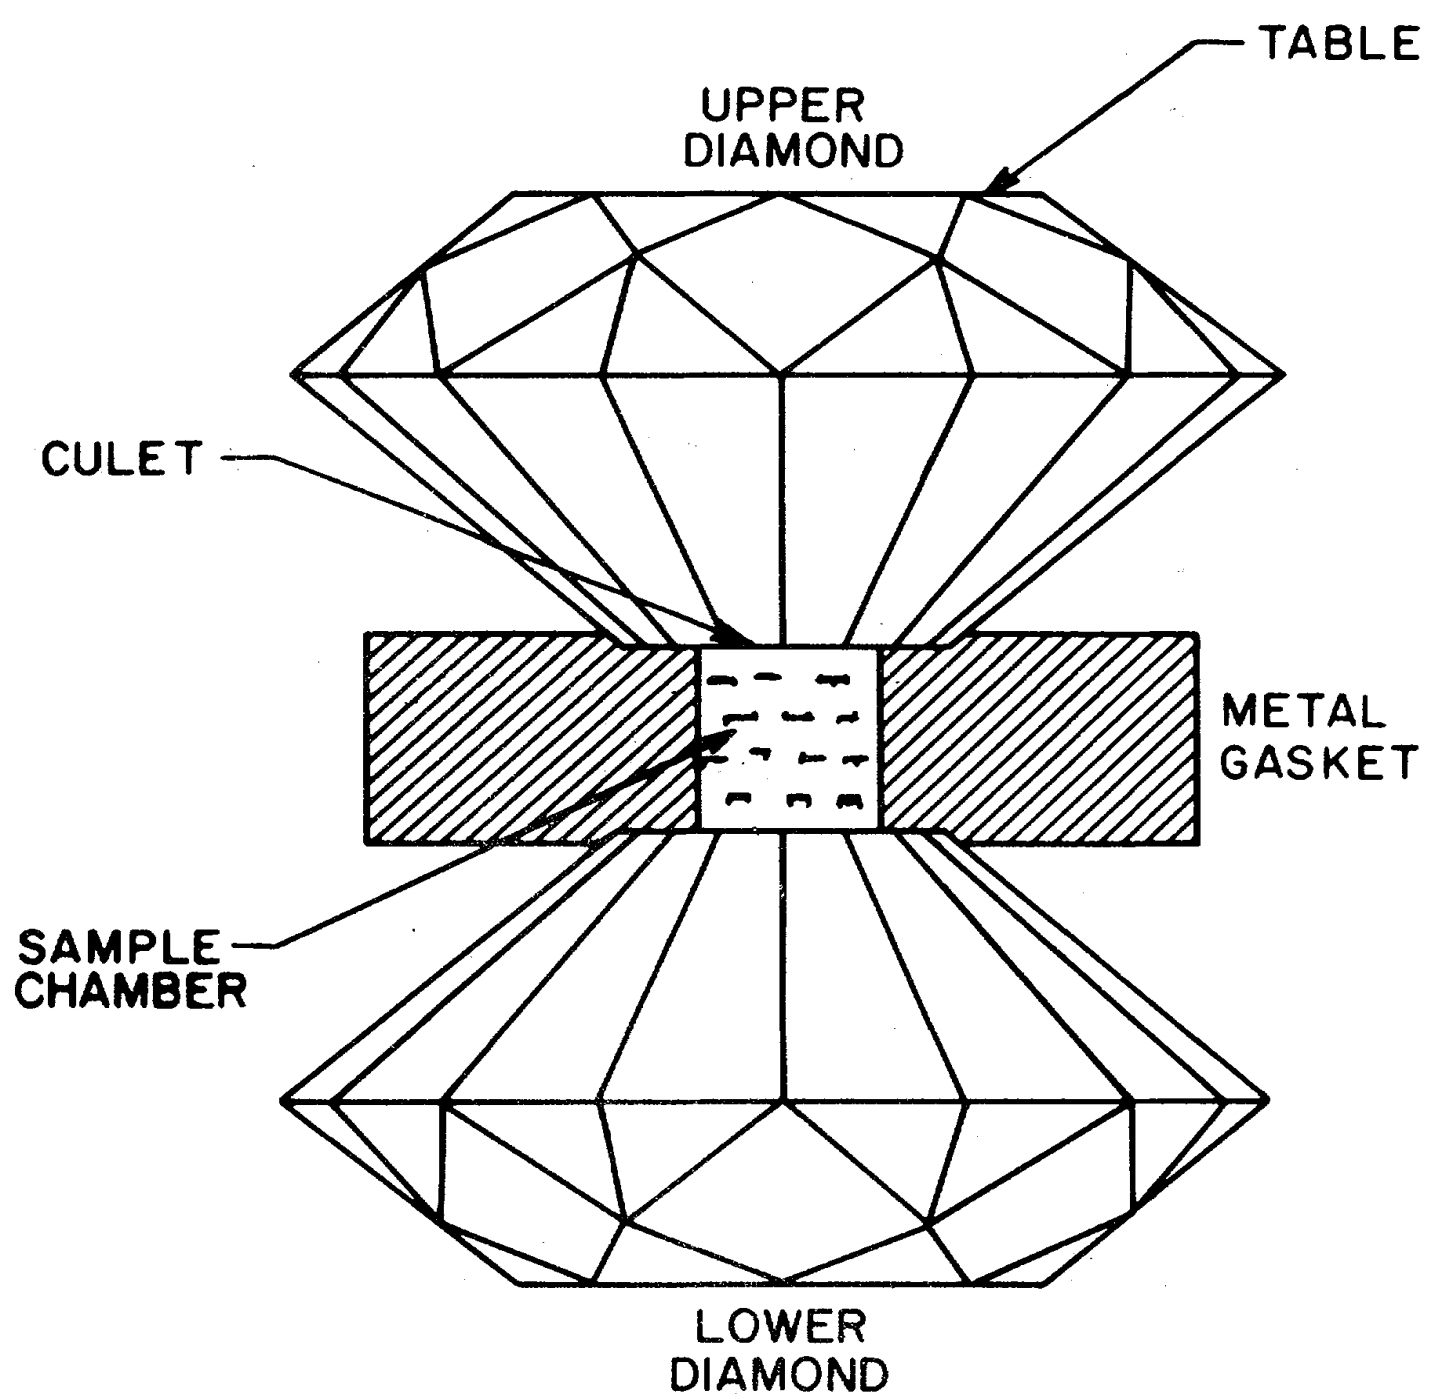
\includegraphics[width=.5\columnwidth]{figures/DAC.png}
	\caption{Diagram of a typical anvil cell, taken from \cite{DAC}}
	\label{fig:1}
\end{figure}

Piston-cylinder cells, on the other hand, allow for a larger sample space, so any transitions of said samples are much easier to notice and measuring resistivity or susceptibility is much easier as well. The only issue with these cells is the pressure regimes they can reach, as the practical pressure limit is around 3 GPa and are often not used up to such regimes.\cite{expmethods}\\

The final type of cell we are interested in is the Indentation cell, depicted in Figure \ref{fig:3}. These types of cells use an anvil made for a hard material like diamond or Tungsten carbide to press and plastically deform a gasket made of an alloy. The anvil would compress into a sample hole in the gasket, as higher pressures are applied, the gasket would yield rather than crack, thus pressurizing and sealing the sample space. This method tends to allow for higher operating pressures than hydrostatic cells, yet has a large sample space so magnetic measurements can be done with more ease than anvil cells.\cite{IndenterCell}

\begin{figure}[ht]
	\centering
	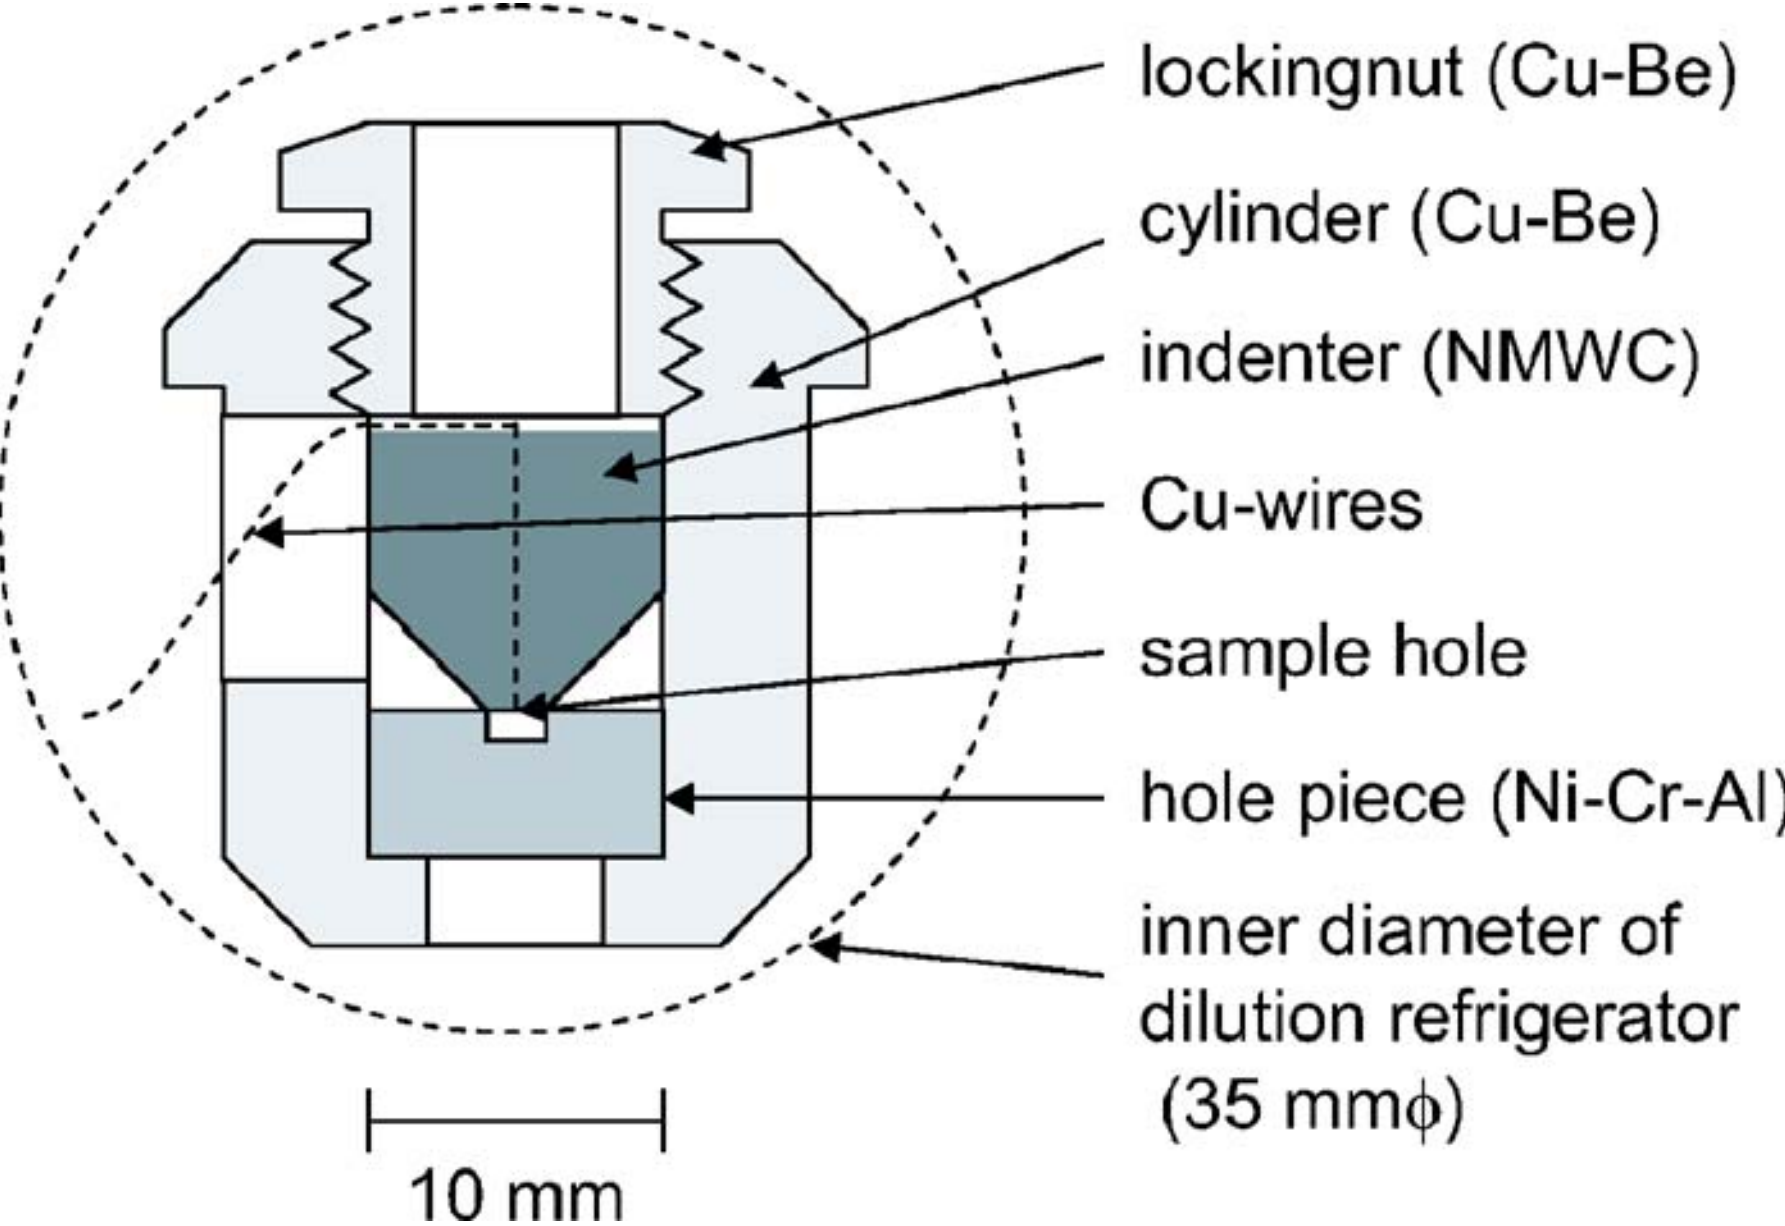
\includegraphics[width=.5\columnwidth]{figures/Indenter_cell.png}
	\caption{Diagram of a typical Indenter cell, taken from \cite{IndenterCell}}
	\label{fig:3}
\end{figure}

\subsection{Methods of probing material properties}

While pressures can be applied on a sample, if information on said sample cannot be obtained, the endeavor to pressurize is all in vain. There are still many methods that can capture the behavior of materials even under high pressures. This section will illustrate some of these relevant methods.

\subsubsection{Magnetic properties}

Magnetic properties are one of the characteristics that can be probed with the use of an external magnetic field. If a sample that undergoes a phase transition were in such a field, the sample would respond depending on its magnetic ordering. If; for example, a material were to go superconducting at a given pressure and temperature, the material would expel all the magnetic flux within it due to the Meissner effect and appear to be a perfect diamagnet, resulting in a sharp drop in the magnetic susceptibility.\cite{diamagnetism}\\

A popular method to collect this information is with the use of AC susceptibility measurements, where a coil is placed around a sample and an AC signal is used, creating a changing magnetic field.\cite{ACsusceptibility} This is done usually by using two coils of wire with roughly equal numbers of turns, when a current is driven through one coil, which we will call the drive coil, a current will be induced on the other, which we will call the pickup coil, due to mutual inductance:

\begin{equation}
M_{DP}=\frac{N_P\Phi_{DP}}{I_D}
\end{equation}

Where $N_P$ is the number of turns of the pickup coil, $\Phi_{DP}$ is the flux from the drive coil to the pickup. If a superconducting sample were place within the drive coil, the Meissner effect would expel any flux within the sample, thus reducing the flux ($\Phi_{DP}$) that can be used to induce a current on the pickup coil. This is observed as a drop in the voltage of the pickup coil.

\subsubsection{Resistivity}

Resistive properties of a material change as a function of temperature. Kinks in these trends can signify structural or electronic transitions and are a useful tool in probing a transition. As an example, $SnTe$ undergoes a structural transition at 97K from cubic to rhombohedral, such a change affects the resistivity significantly, as in Figure \ref{fig:5}. As seen here, there is a significant change in resistivity as this transition occurs. Other transitions such as that of superconductivity have equally distinctive features, as will be discussed later.\\

\begin{figure}[ht]
	\centering
	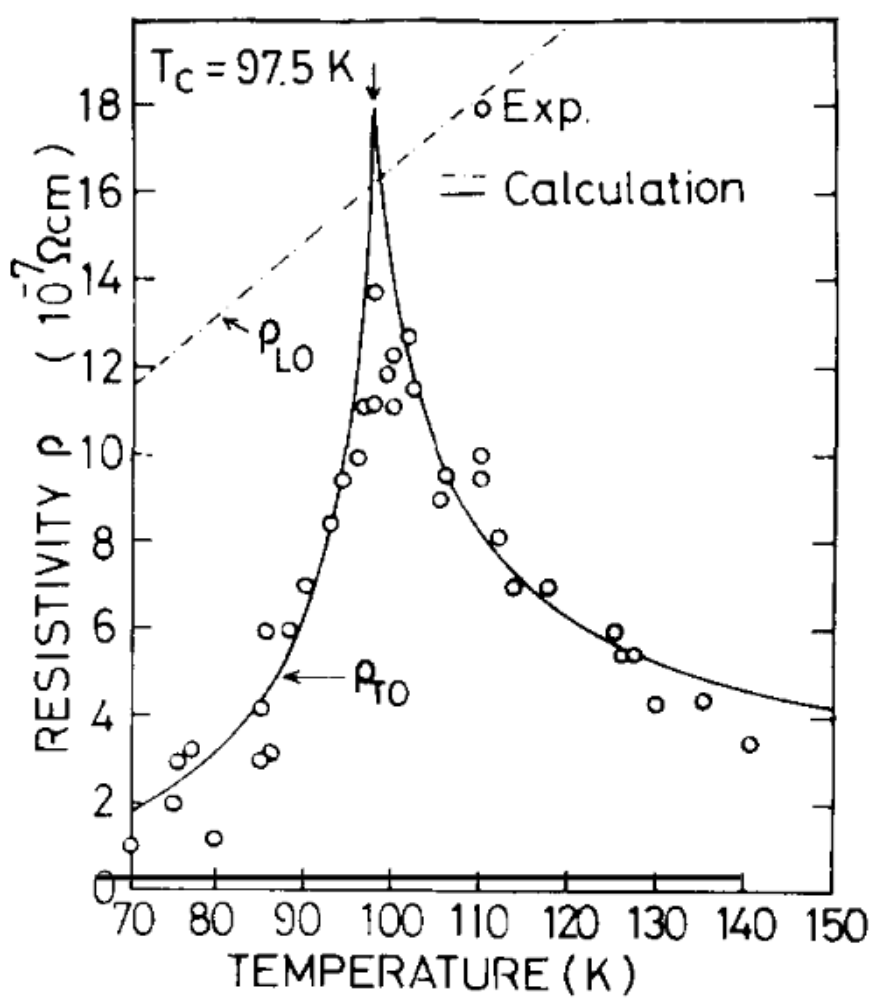
\includegraphics[width=.425\columnwidth]{figures/resistivity.png}
	\caption{Resistivity over temperature plot around the structural transition for $SnTe$ taken from \cite{resistivity}}
	\label{fig:5}
\end{figure}

The most common method of measuring resistivity is using the 4-terminal method, where the voltage and current across a sample is measured and Ohm's law is used to determine resistance. If this is done under pressure, it is standard to measure the resistance of another material whose transition temperature changes with pressure and is well known, like lead.

\subsection{Motivation for a new cell design}
\label{sec:motivation}

As mentioned previously, FBBO was studied by a PhD student, some odd features were found, including a hysteresis loop which can be found in Figure \ref{fig:10} and another being an anti-ferromagnetic (AFM) phase that leads to a quantum critical point (QCP) in Figure \ref{fig:11}. First considering the phase diagram, an AFM phase was observed, but only two points were used to constrain this phase. More points can be gathered to better map the phase space, which is one of the reasons a cell that can collect magnetic susceptibility data at intermediate pressures is necessary.

\begin{figure}[ht]
	\centering
	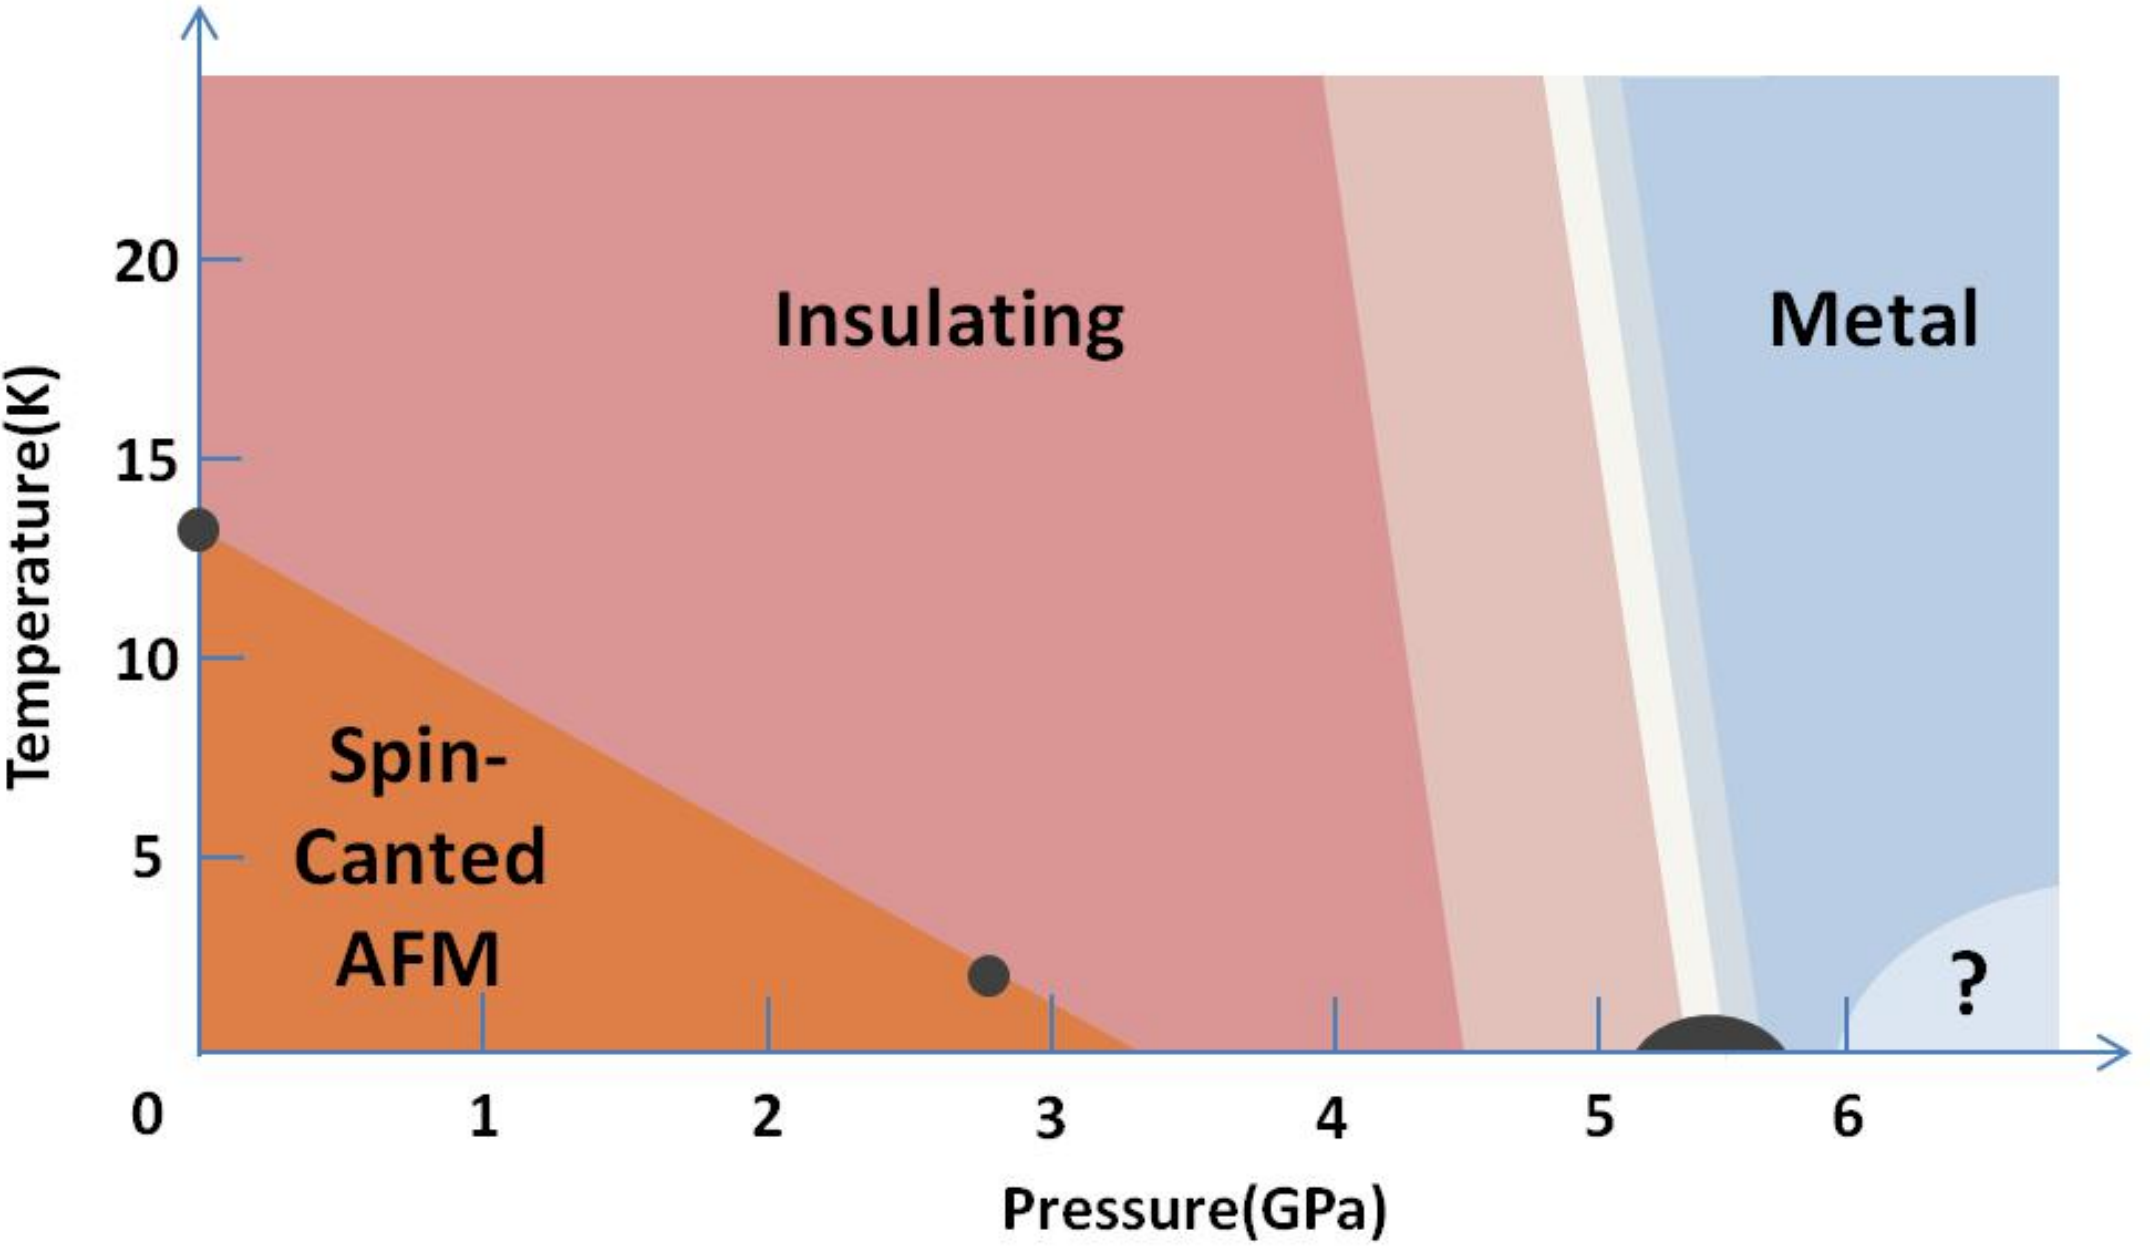
\includegraphics[width=.7\columnwidth]{figures/phase_diagram.png}
	\caption{Rough phase diagram showing an anti-ferromagnetic phase taken from \cite{Di_thesis}}
	\label{fig:11}
\end{figure}

The reason the phase diagram shows a spin-canted AFM is due to the crystal structure and orientation of the FBBO molecules, as can be seen in Figure \ref{fig:12}. FBBO is arranged in layers, where \ref{fig:12}b shows the spin orientations along a single layer, which looks like a ferromagnet. While in \ref{fig:12}c, the spins are oriented like a spin canted anti-ferromagnet, as the spins are not exactly anti-parallel to one another. At temperatures and pressures where the AFM state is found, the anti-ferromagnetic state is dominant.\\

\begin{figure}[ht]
	\centering
	\subfigure{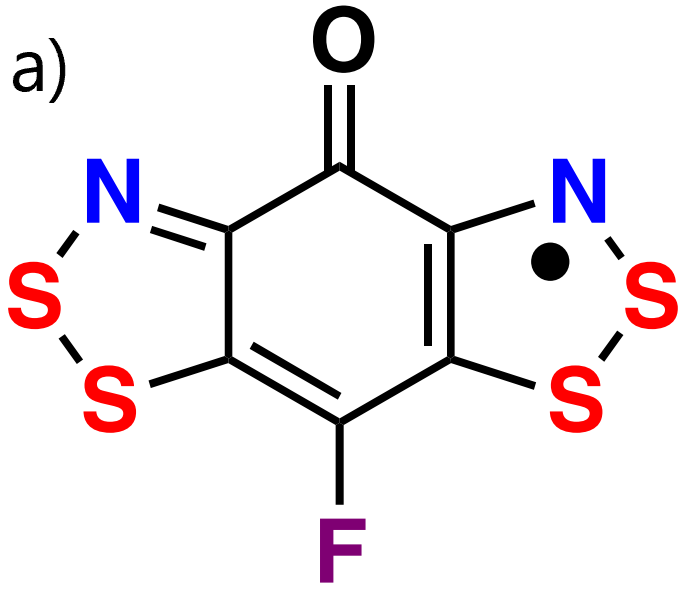
\includegraphics[width=.3\columnwidth]{figures/FBBO.png}}
	\hspace{2mm}
	\subfigure{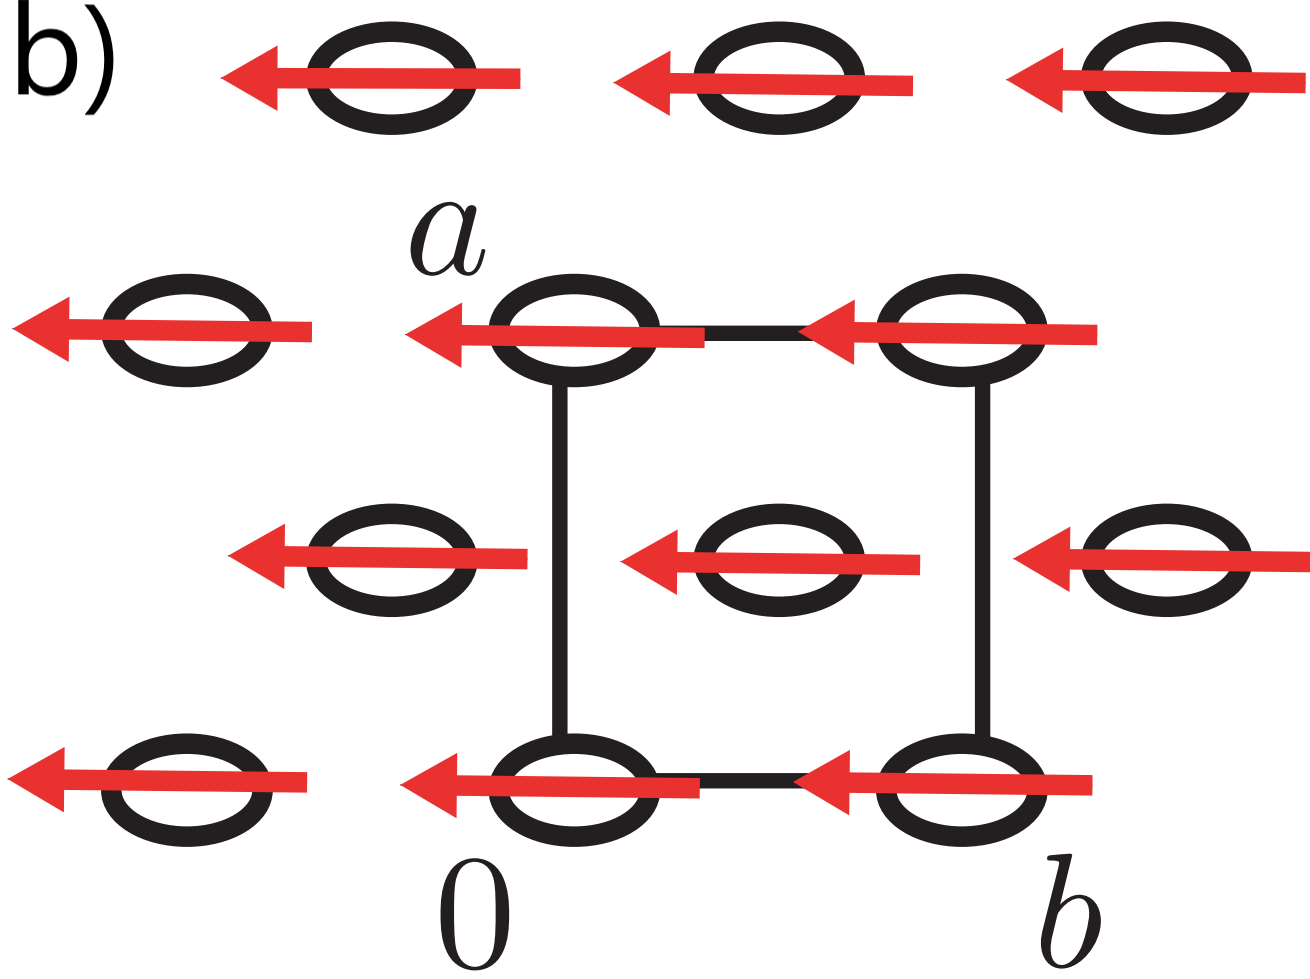
\includegraphics[width=.3\columnwidth]{figures/FBBOab.png}}
	\hspace{2mm}
	\subfigure{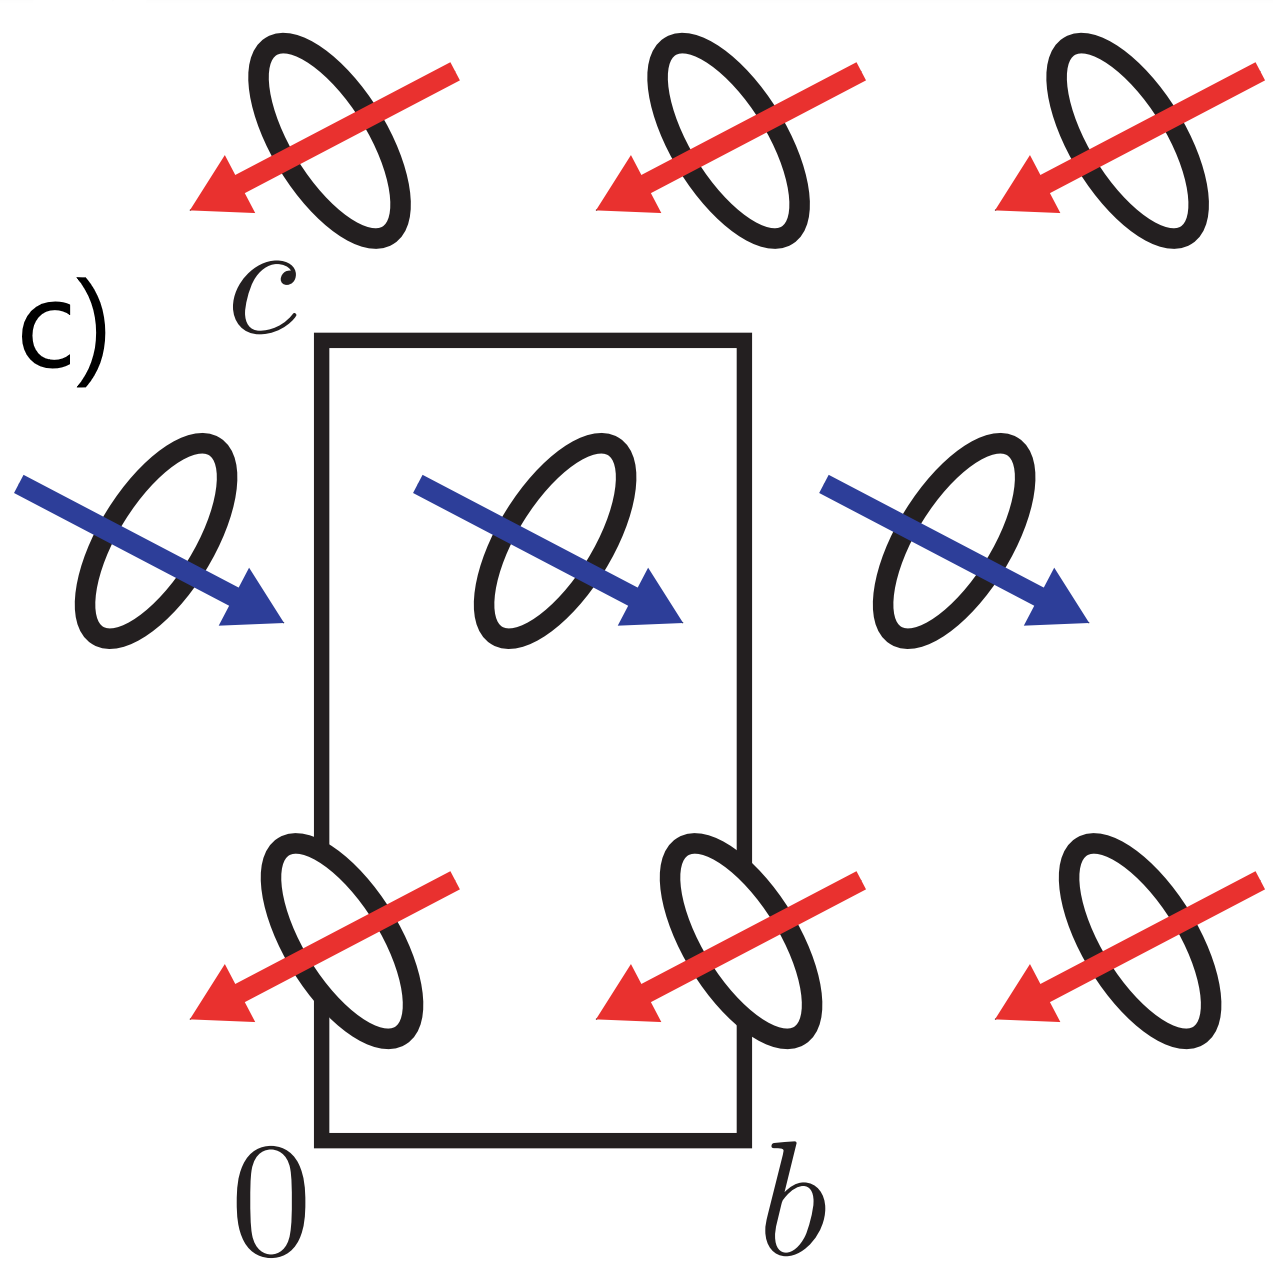
\includegraphics[width=.3\columnwidth]{figures/FBBOcb.png}}
	\caption{Structure and arrangement of FBBO molecules in a lattice with the preferred direction of spin as depicted by the colored arrows, taken from \cite{FBBO}}
	\label{fig:12}
\end{figure}

The hysteresis loop in Figure \ref{fig:10} shows the resistivity as measured with an increasing DC magnetic field at 2.6GPa. The magnetic field strength was changed from 0T $\rightarrow$ 5T $\rightarrow$ 0T $\rightarrow$ -5T $\rightarrow$ 0T in that order for the runs at 500 and 50mK. Changing the field strength in such a way showed how resistivity is dependent on the manner in which the magnetic field changes, which is called hysteresis. As temperature was lowered beyond 1.2K, the hysteresis becomes more pronounced.\cite{Di_thesis}\\

\begin{figure}[ht]
	\centering
	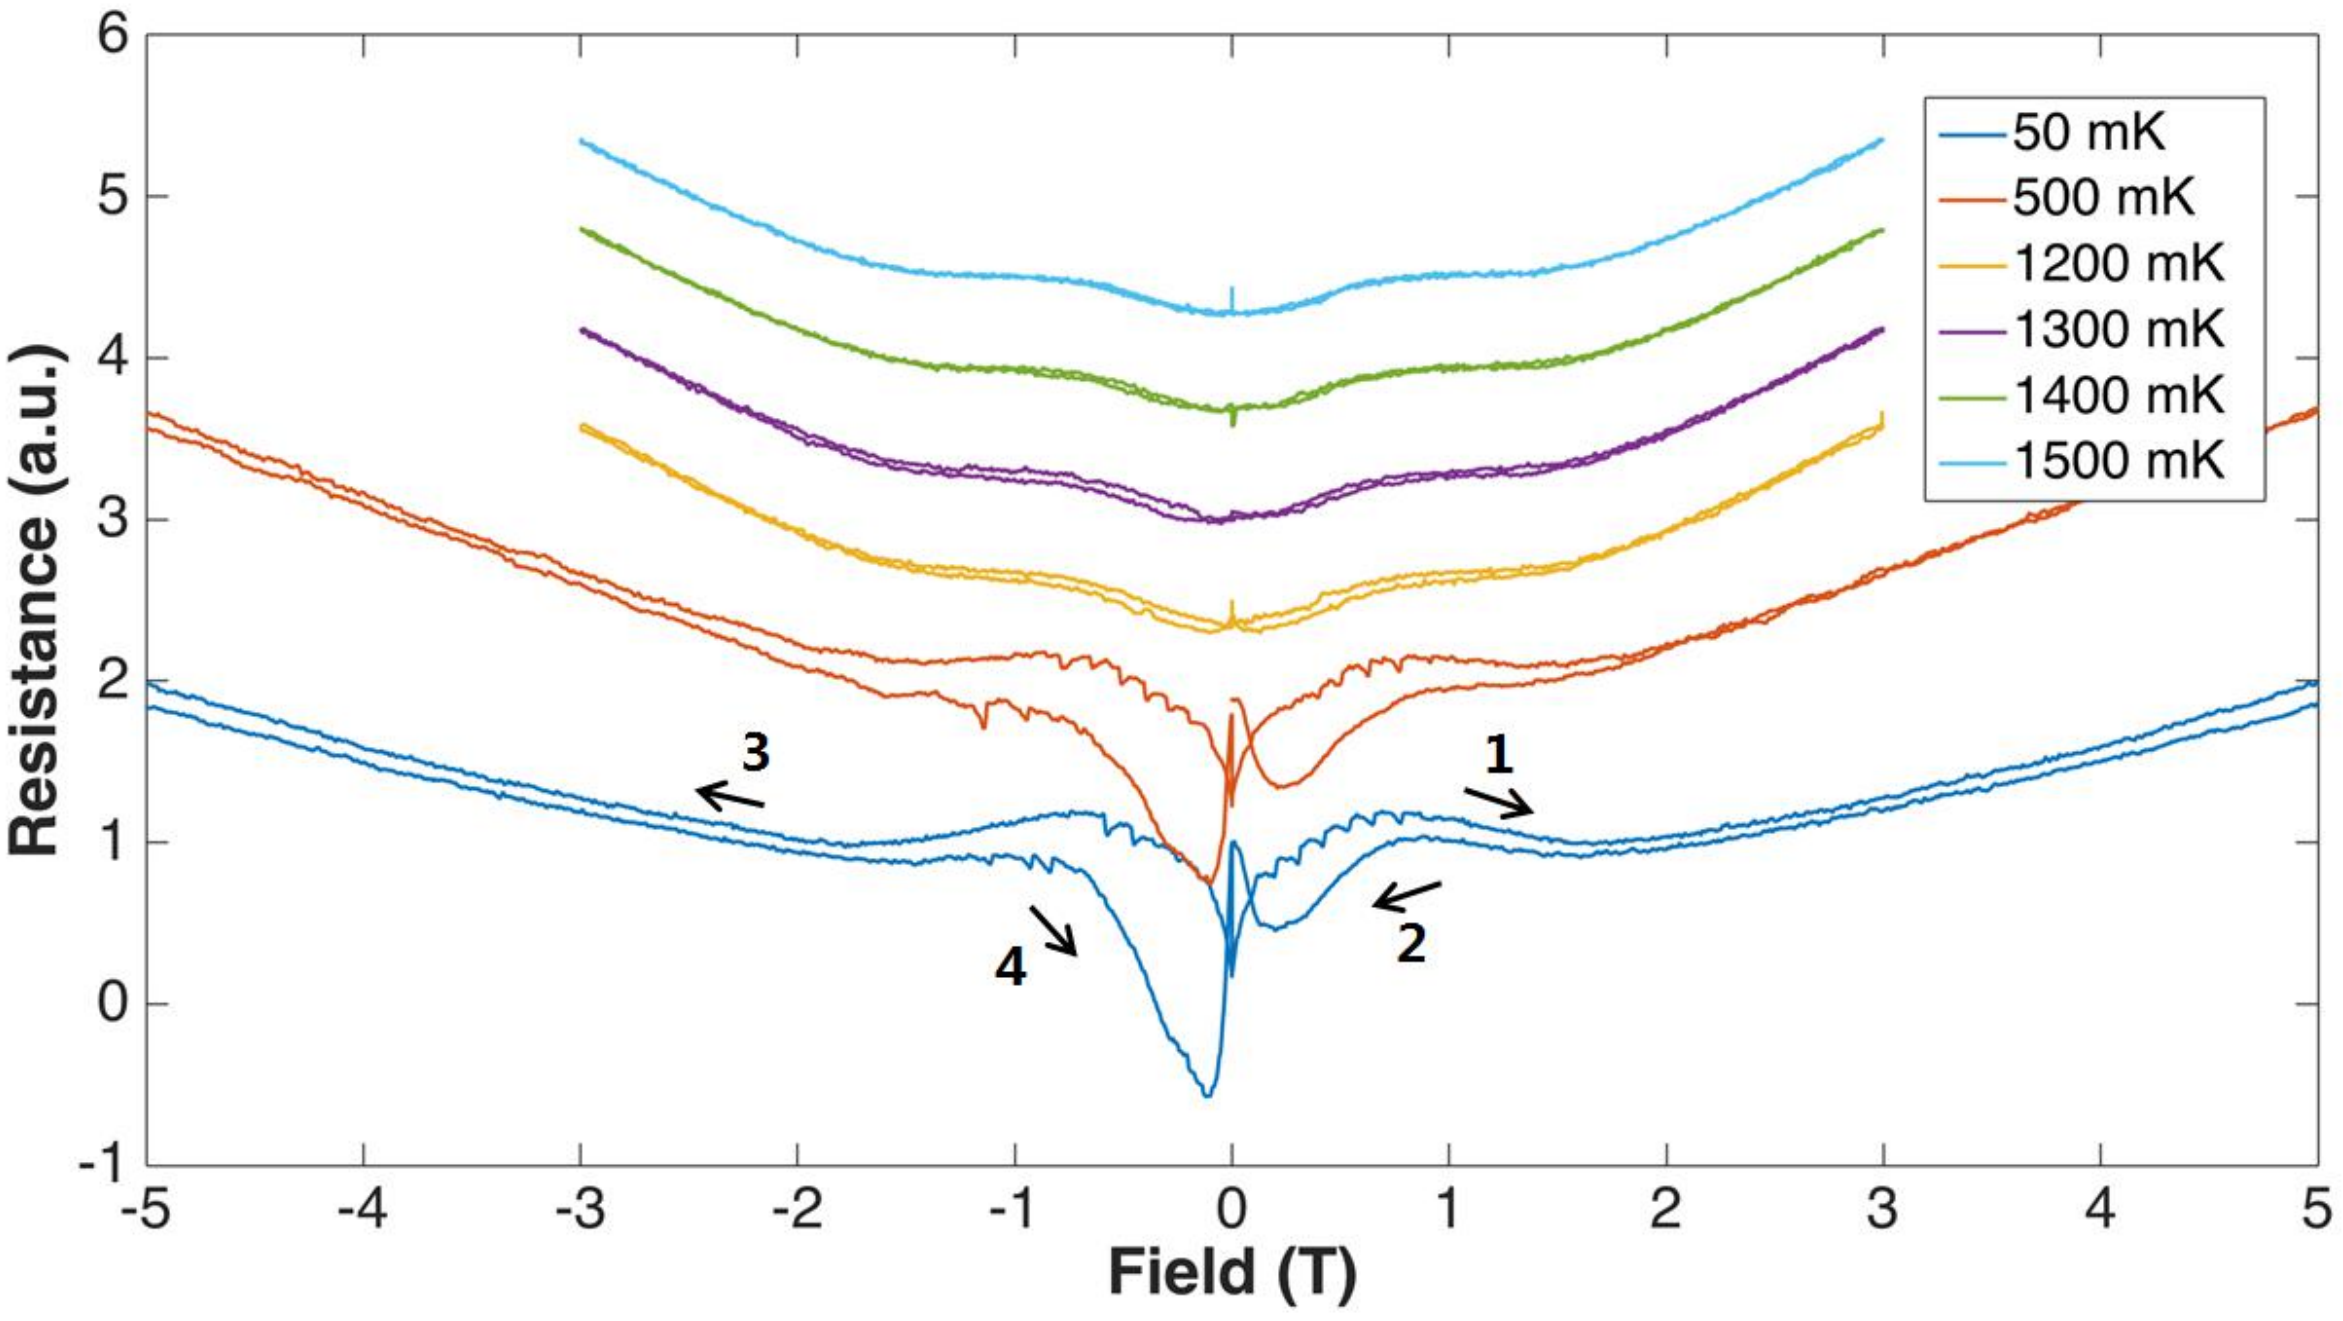
\includegraphics[width=.7\columnwidth]{figures/hysteresis.png}
	\caption{Hysteresis loop from a resistivity measurement on FBBO, taken from \cite{Di_thesis}}
	\label{fig:10}
\end{figure}

The explanation behind why this occurs is not fully known, but it is likely due to the spin orientations of the FBBO and how a current flows through it. If a larger sample of FBBO were to be put under a similar amount of pressure, magnetic susceptibility measurements could be done to better understand the situation, which is why it is important to make a cell such as the indenter cell.

\section{Project Design}

The design for the Indenter cell proposed here was based on a cell described in \cite{IndenterCell}. This section will discuss the previous design and how it holds pressure, then the modifications made and their reasoning.

\subsection{Original Design}

A design of the previous Indenter cell can be found in Figure \ref{fig:4}. This cell uses an anvil made of Tungsten Carbide with a feed through hole for wires from a coil, which rests in the sample space. Tungsten Carbide is used in this instance due to its large Young's modulus, which allow the anvil to sustain high pressures without cracking or deforming.\\

The anvil would indent onto a gasket made of Nickel-Chromium-Aluminum, which is an appealing material primarily due to its low temperature dependence on resistivity and magnetic susceptibility.\cite{expmethods} Its properties as an alloy is useful as well, since the gasket would plastically deform when pressed by the anvil, thus holding pressure rather than cracking. Within the sample space, Daphne Oil is used as a pressure medium to hydrostatically apply pressure on a sample.\\

A drive and pickup coil is used to collect data on the magnetic susceptibility of a sample, the wires for which are fed through the anvil itself around a cone seal. This cone seal is surrounded by stycast, which is a strong epoxy that can hold pressure well and protect the thin copper wires from being severed under high pressures.

\begin{figure}[ht]
	\centering
	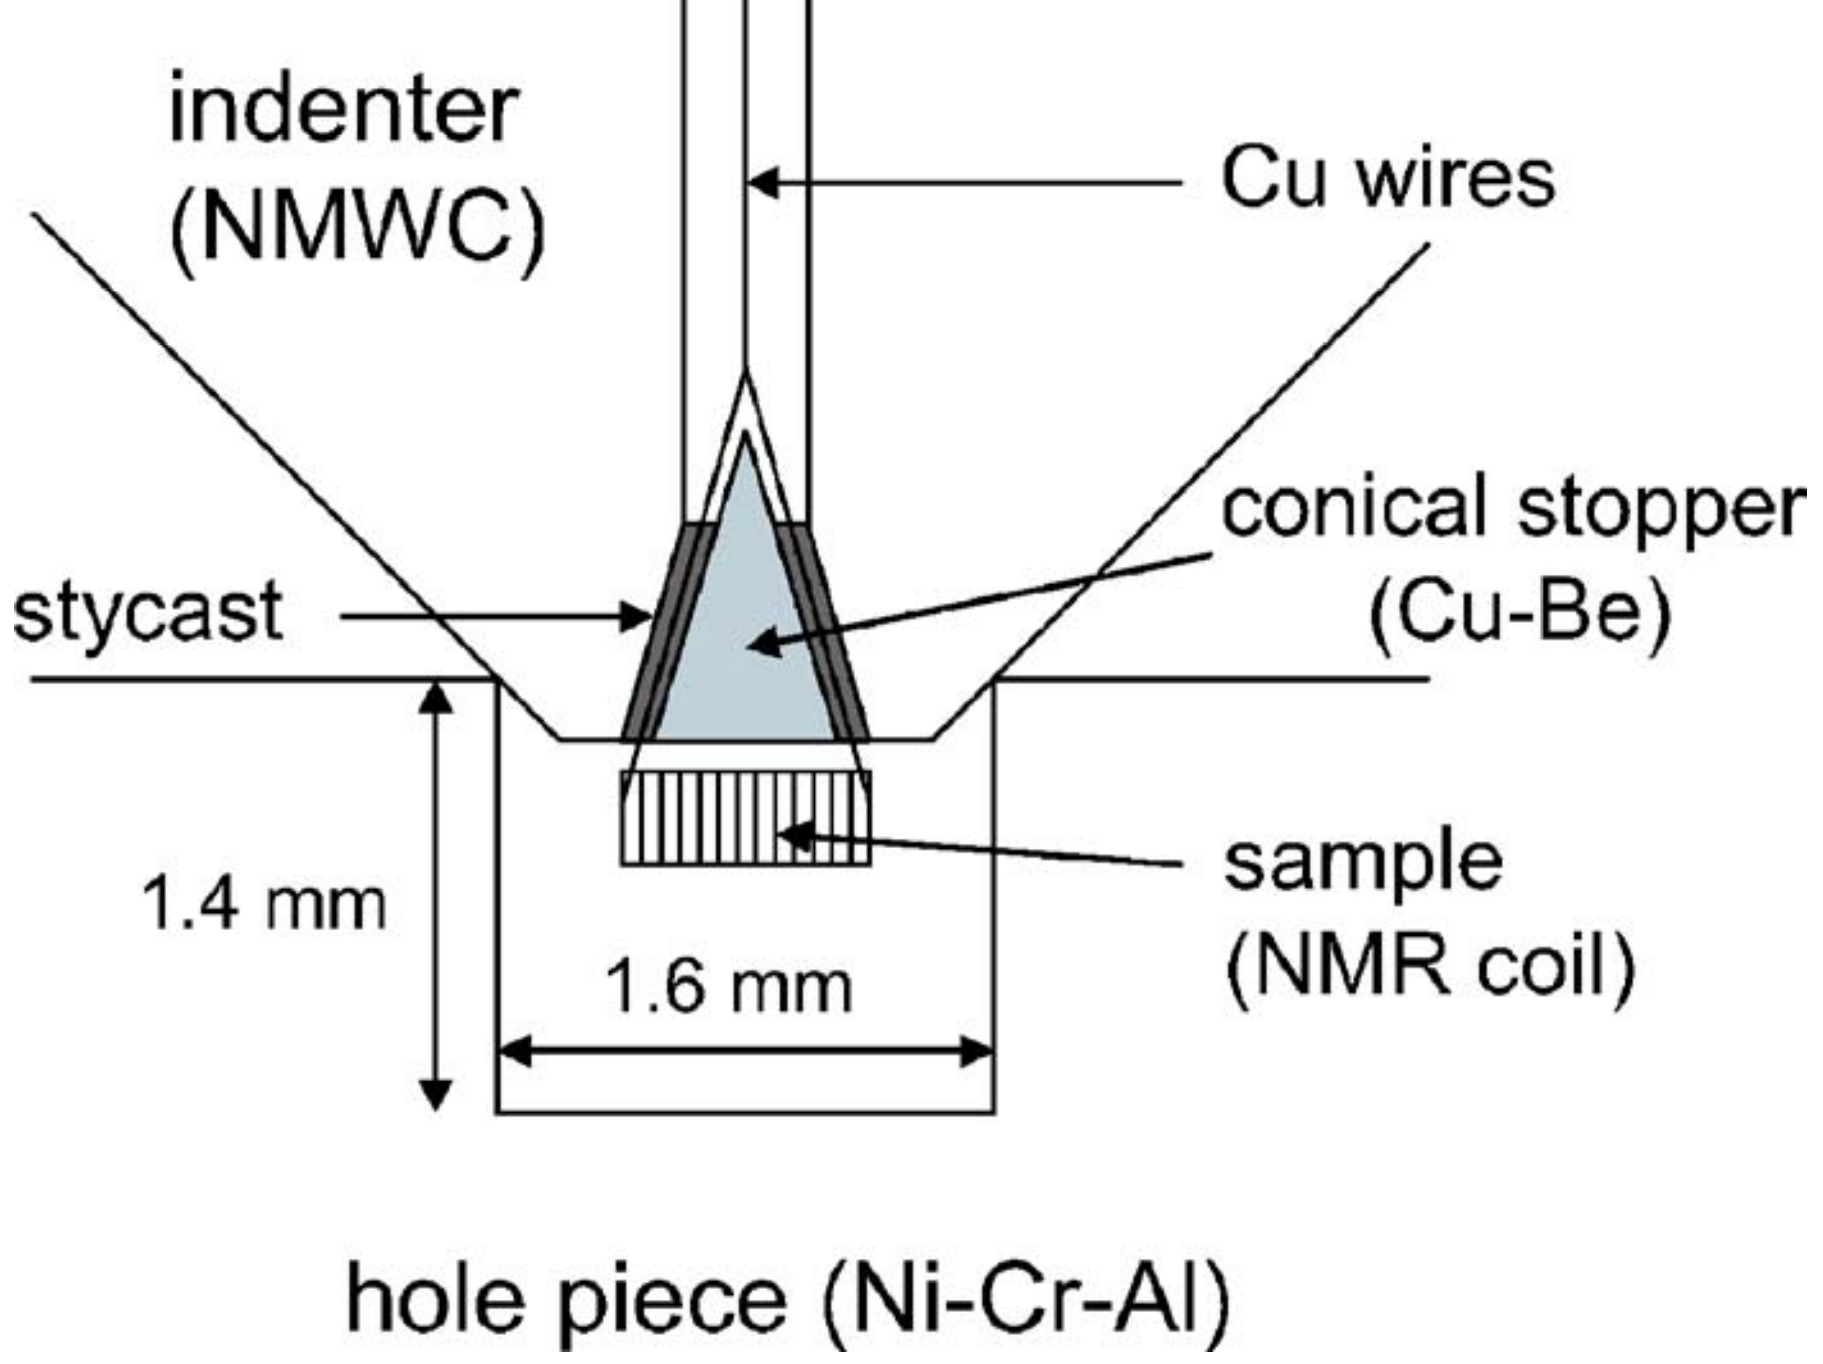
\includegraphics[width=.5\columnwidth]{figures/old_cell.png}
	\caption{Indenter cell design take from \cite{IndenterCell}}
	\label{fig:4}
\end{figure}

This design with the Daphne Oil can reach pressures  of up to 4.5 GPa\cite{IndenterCell}, the design proposed in this paper should be able to reach similar pressure with some modifications. These modifications are necessary, as previous attempts using such a design were unsuccessful due to the sensitive wires being severed.\\

\subsection{Modified Indenter Cell}

The modified design should be able to achieve the same pressure regimes at a lower cost over multiple uses and utilizes a balance coil, which reduces any noise present. A diagram of the cell can be found in Figure \ref{fig:2}. The changes made to the original design include the use of a balance coil, placement of sample coil, expansion of sample space and the use of a different material for the gasket (MP35N), which has similar magnetic qualities to Ni-Cr-Al.\cite{IndenterCell}\cite{MP35N_similarities}\\

\begin{figure}[ht]
	\centering
	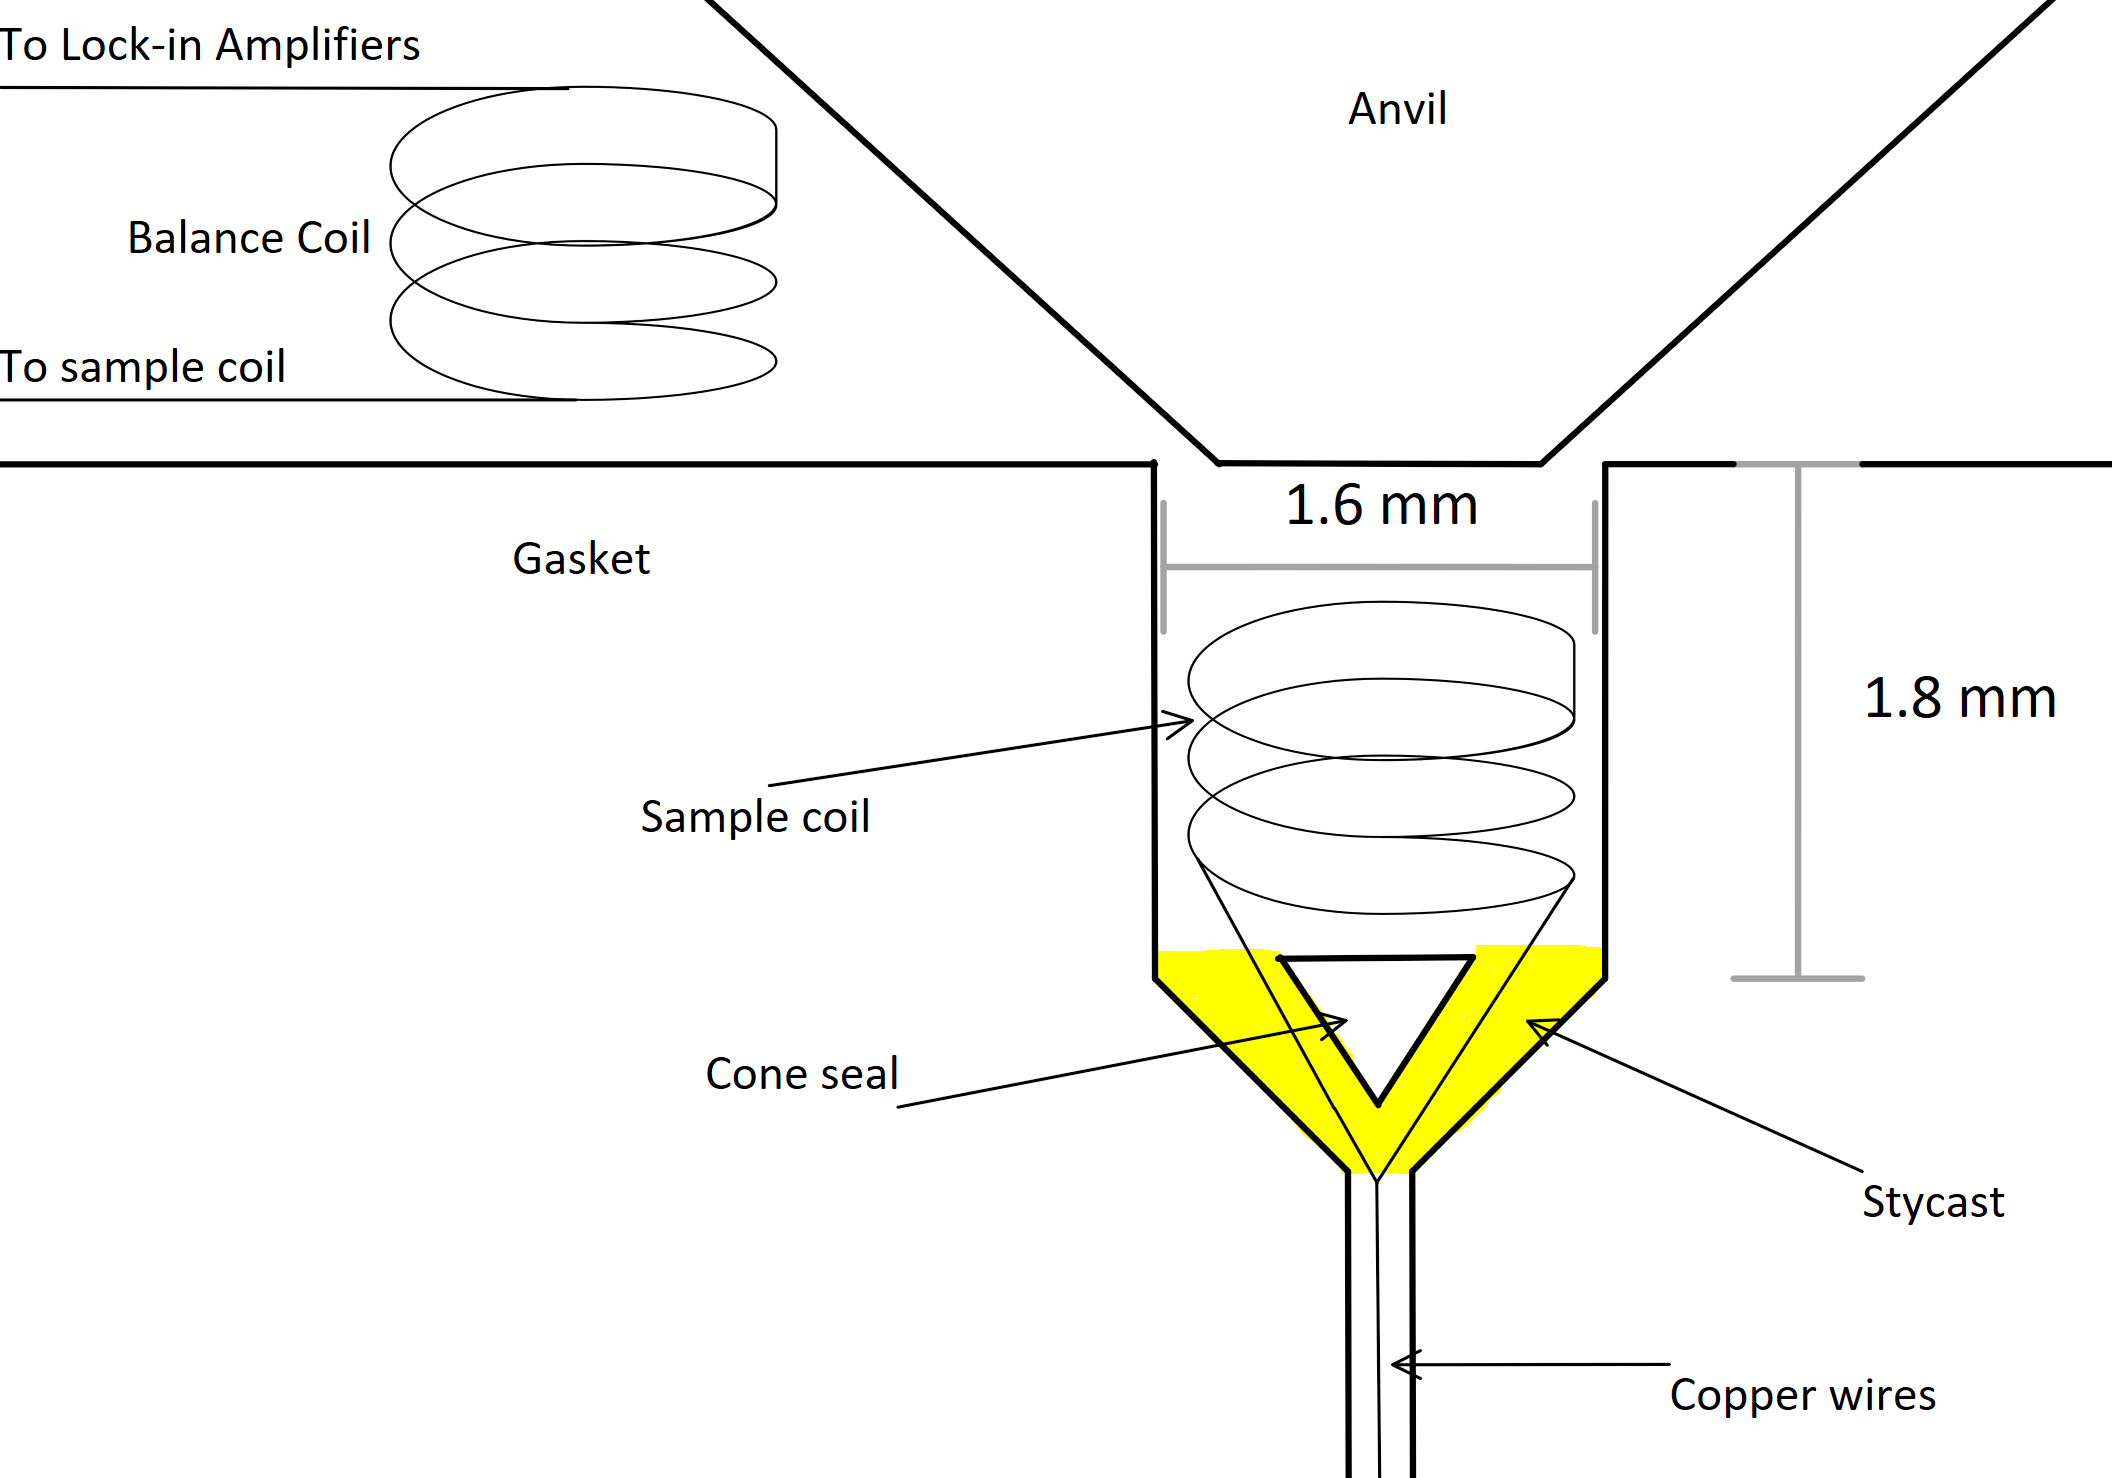
\includegraphics[width=.6\columnwidth]{figures/Modified_Indenter_Cell_Design.png}
	\caption{Modified Indenter cell design}
	\label{fig:2}
\end{figure}

The new placement of the sample coil allows the wires to be better protected during setup of the apparatus, since 25 $\mu$m wire is used to make the coil. Along with that, it is easier to place samples within the coil in such an orientation. Regarding the coils themselves, the sample and balance coil are comprised of two coils, the drive coil and a pickup wrapped around the drive. The drive in the sample coil is connected in series with the drive in the balance coil, while the pickups of each are connected in anti-series. This is done to reduce the noise that is collected by the pickup coils, as will be discussed in section \ref{sec:coils}. The drive coil is supplied with a voltage and the pickup is connected to a Lock-in amplifier and its voltage is monitored, so any deviation can be considered to be due to the sample itself.\\

The sensitivity of the coils are dependent on the magnetic flux they produce as current is run through them as follows,

\begin{equation}
	\Phi = \vec{B}\cdot\vec{A} = \frac{\mu_0N_DI_DA}{L}
	\label{eq:2}
\end{equation}

Where $\vec{A}$ is assumed to be in the same direction as $\vec{B}$, $\mu_0$ is the permeability of free space and $L$ is the length of the coil. While current is supplied to create a magnetic field, this also creates some heat and since measurements with these coils are done at low temperatures, the heat produced can be important. In our case the heat produced by the coils are on the order of milliKelvin, so don't create a significant effect.

\subsection{Coil Wiring}
\label{sec:coils}

The balance and main coils need to be connected in a manner that would cancel out any noise that exists in the background. This is done by connecting the drive coils in series, while keeping the pickup coils in anti-series, a depiction of this can be found in Figure \ref{fig:7}. A setup such as this reduces noise by canceling voltages collected by the pickup coils. The drive coils both emit a similar amount of flux that is observed by the pickup coils since they have the same number of turns. But since the pickup coils are in anti-series, currents are induced in opposing directions, thus canceling each other. However, if there is a sample within one of the coils which expels magnetic flux, this will create a non-zero voltage that can be collected with a Lock-in amplifier and signify a transition.

\begin{figure}[ht]
	\centering
	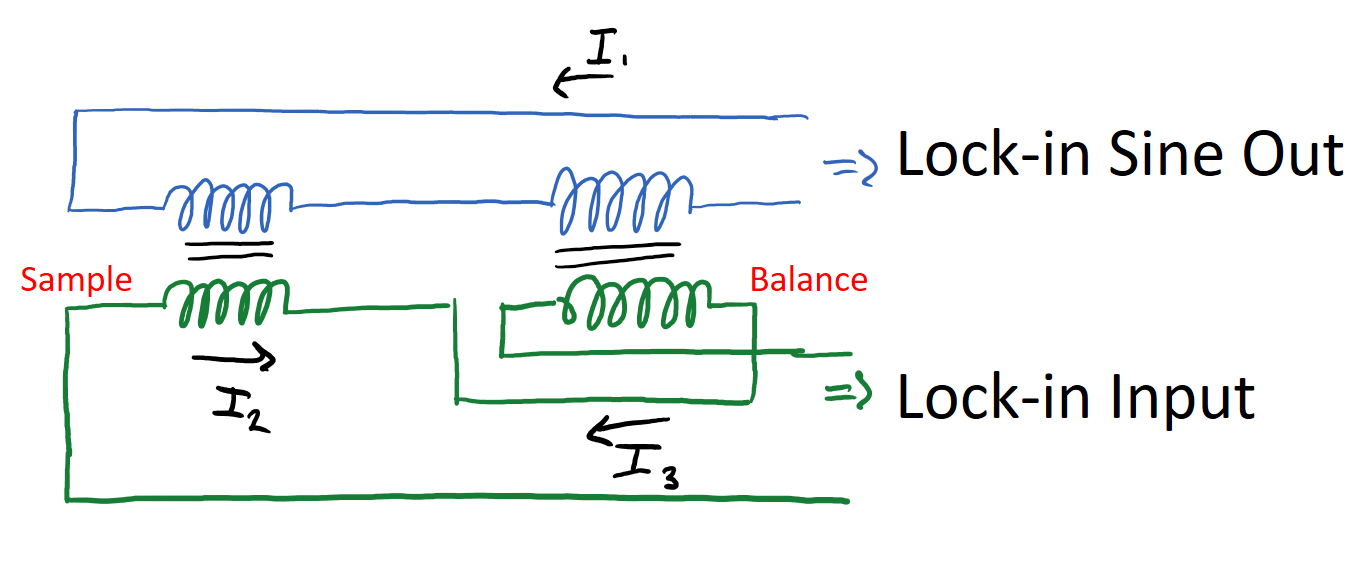
\includegraphics[width=.6\columnwidth]{figures/canceling.png}
	\caption{Balance and Sample coils canceling currents}
	\label{fig:7}
\end{figure}

\subsubsection{Coil Testing}

The setup in Figure \ref{fig:7} requires the tracking of wires, as checking whether a coil is being wrapped clockwise or counter clockwise with respect to a specific orientation can be difficult or impossible at times. A test needs to be used to confirm the connection of the coils is correct, a scheme of the testing circuit can be found in Figure \ref{fig:6}. In such a configuration, the drive coils are supplied with an AC current, the pickup coils need to be tested to be in the correct orientation so their voltages sum to close to 0V.

\begin{figure}[ht]
	\centering
	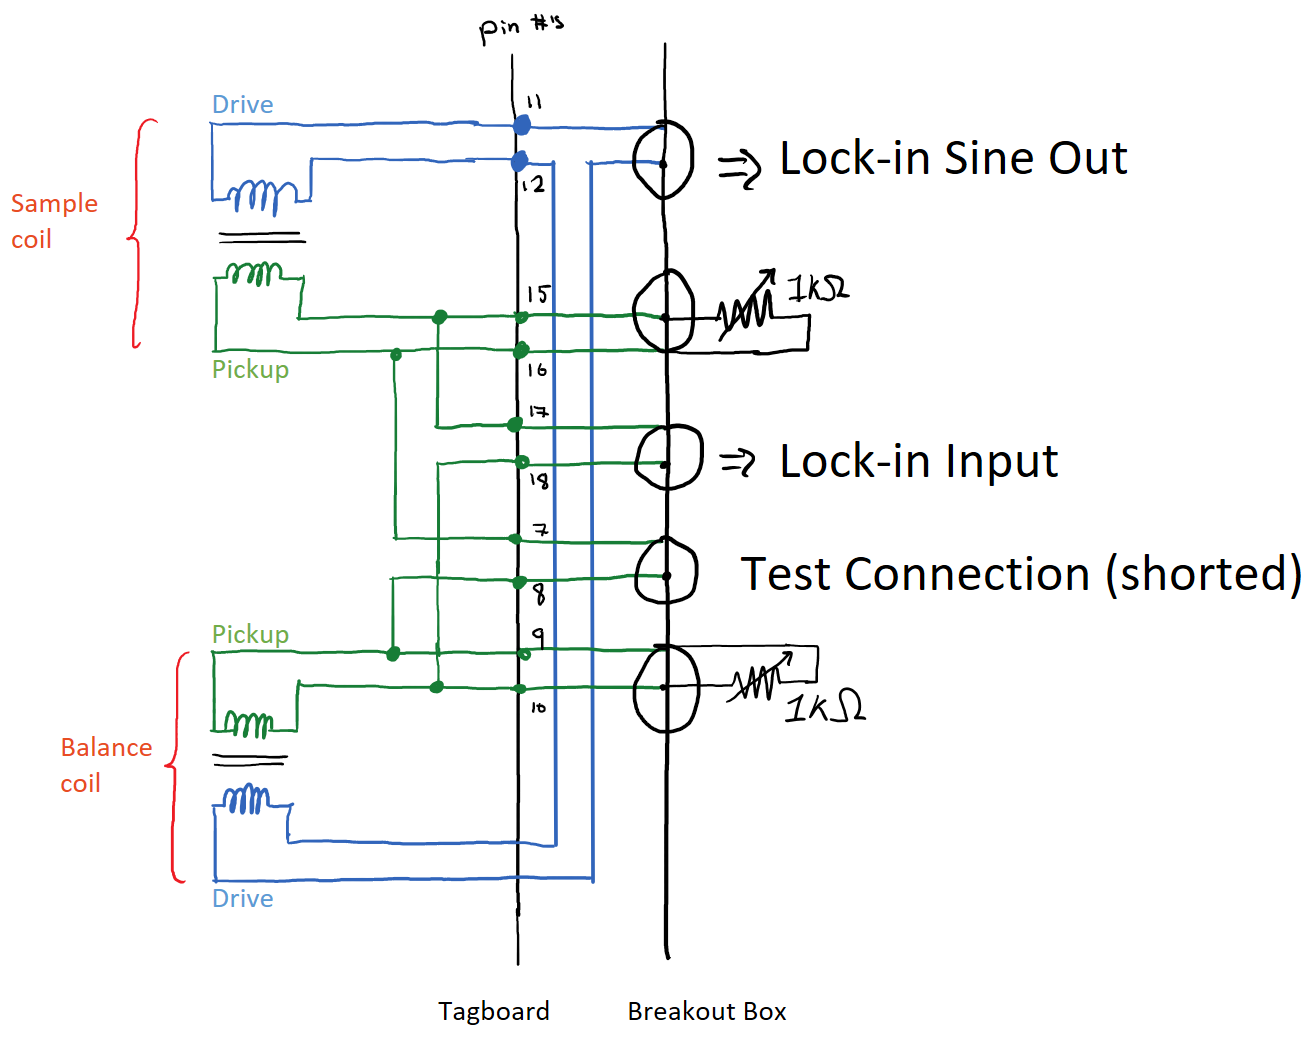
\includegraphics[width=.6\columnwidth]{figures/wiring.png}
	\caption{Wiring scheme between coils}
	\label{fig:6}
\end{figure}

The input from the Lock-in with this circuit would change as the test connection is shorted, the manner in which the signal changes can give insight as to whether the coils are in series or anti-series. If the coil is in series, the signal should fall like in Figure \ref{fig:13}b, while if it's in anti-series, the signal from the Lock-in Input should rise like in Figure \ref{fig:13}a.

\begin{figure}[ht]
	\centering
	\subfigure[Signal from pickup coils in anti-series]{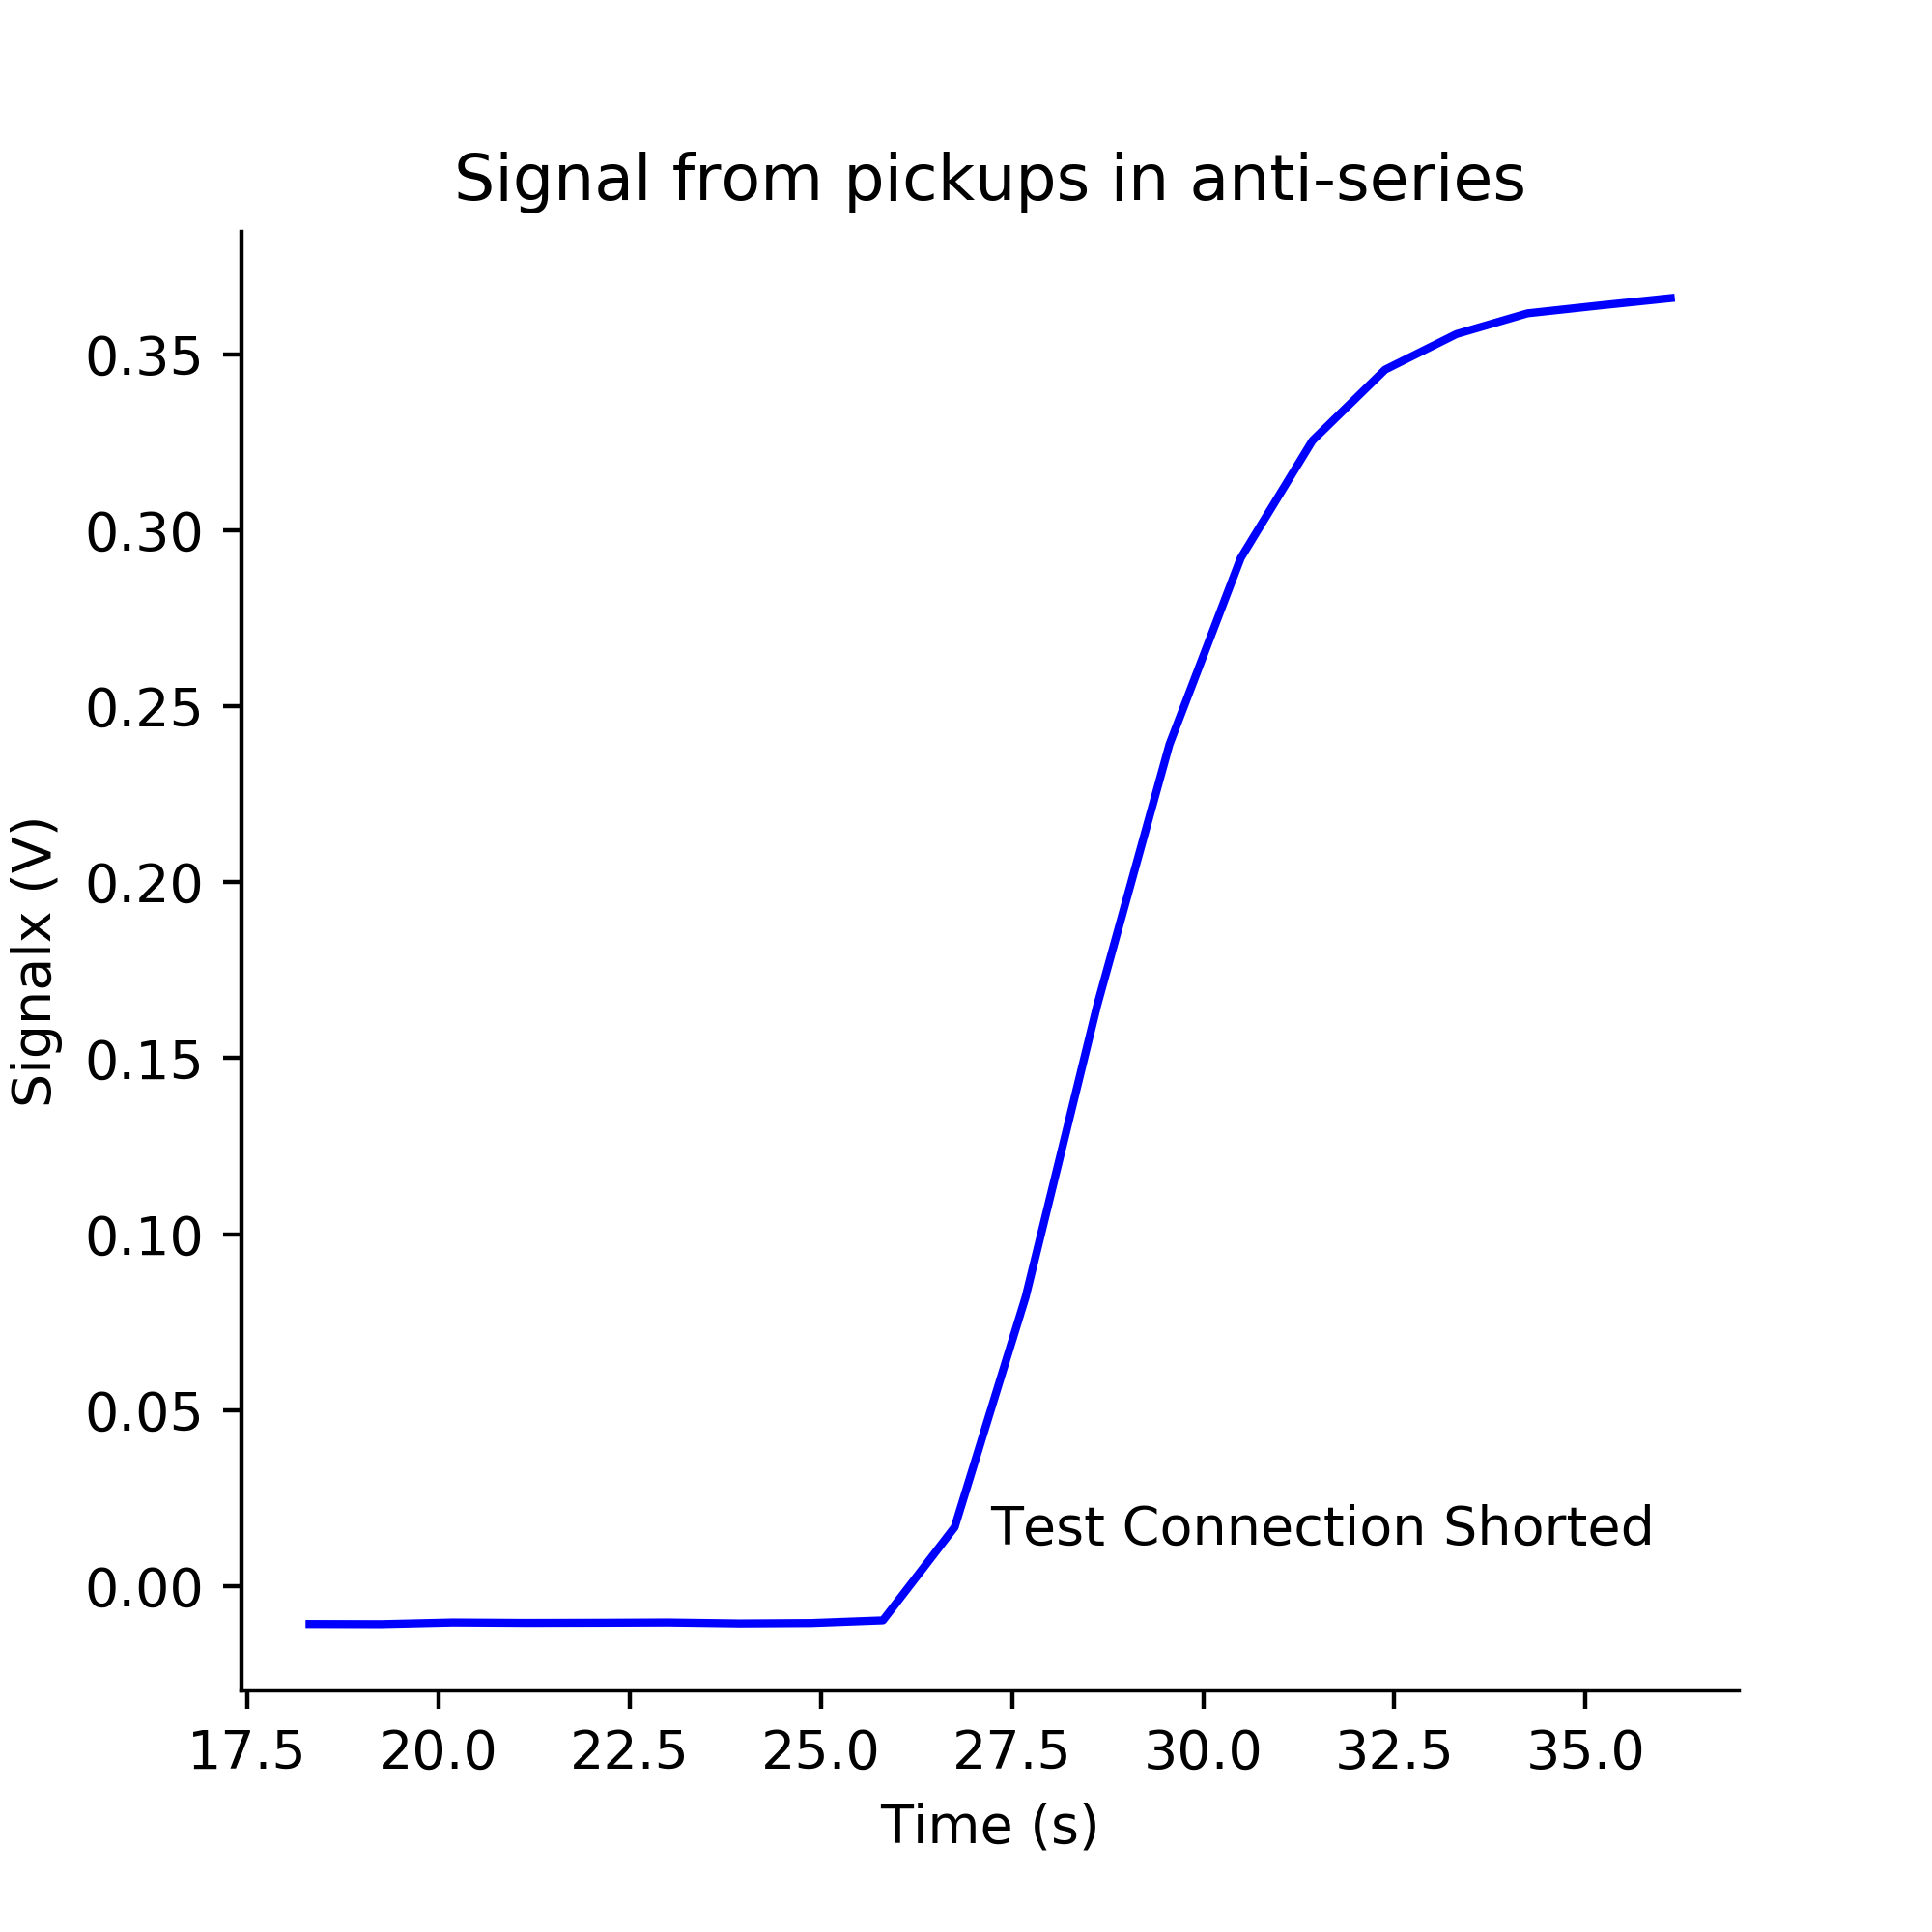
\includegraphics[width=.3\columnwidth]{figures/Antiseries.png}}
	\hspace{5mm}
	\subfigure[Signal from pickup coils in series]{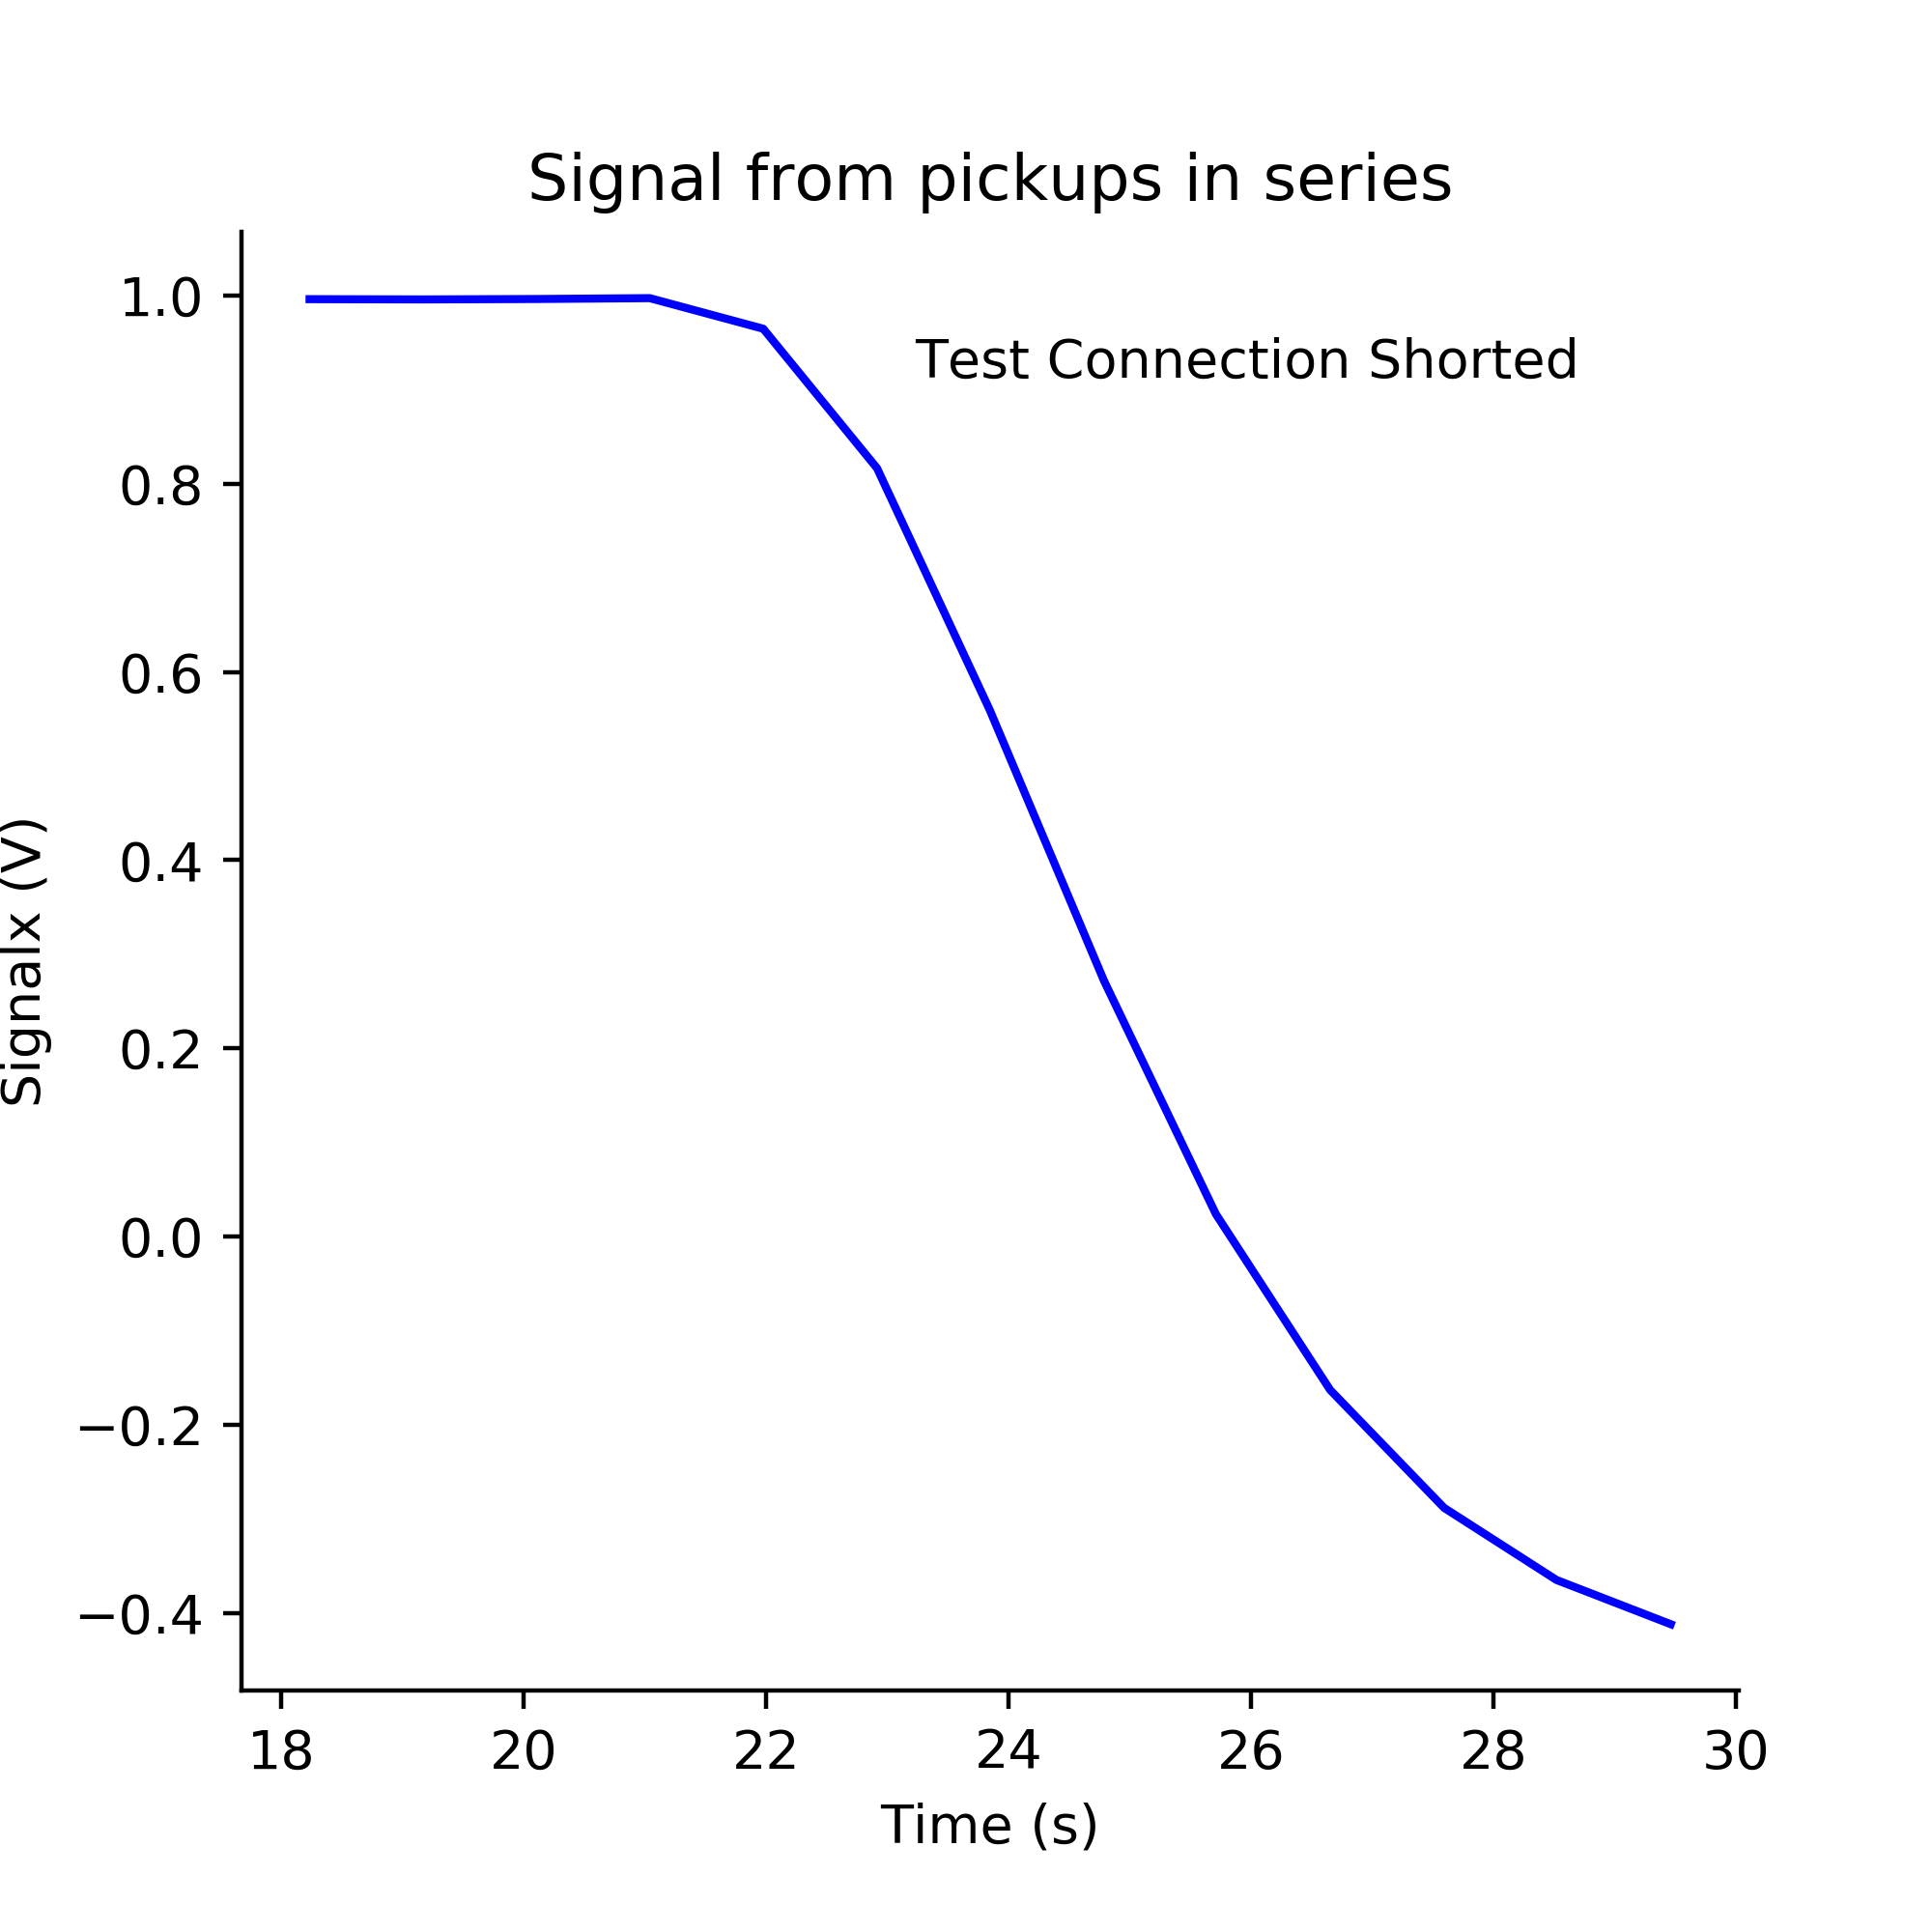
\includegraphics[width=.3\columnwidth]{figures/Series.png}}
	\caption{Signals using the circuit in Figure \ref{fig:6}}
	\label{fig:13}
\end{figure}

\section{Transitions}

To test the cell, a sample whose properties have been thoroughly studied at certain temperature and pressures are necessary. Lead is the perfect candidate for this, as its superconducting transition as a function of pressure is well known and can be found using this cell in Figure \ref{fig:9}. There are a few features of this transition that appear to stand out: the superconducting transition temperature is higher than the expected 7.19K for lead and the shape is not what would typically be expected from a superconducting transition.\cite{lead}\\

The temperature deviation can be explained as being due to the thermometry of the probe attached to the Indenter cell. A Cernox thermometer was used to gather temperature data and the deviation is likely due to a lack of proper thermal contact with its environment. This can be reconciled by using an exchange gas, like Helium to make thermal contact with the thermometer and the Indenter cell itself.

\begin{figure}[ht]
	\centering
	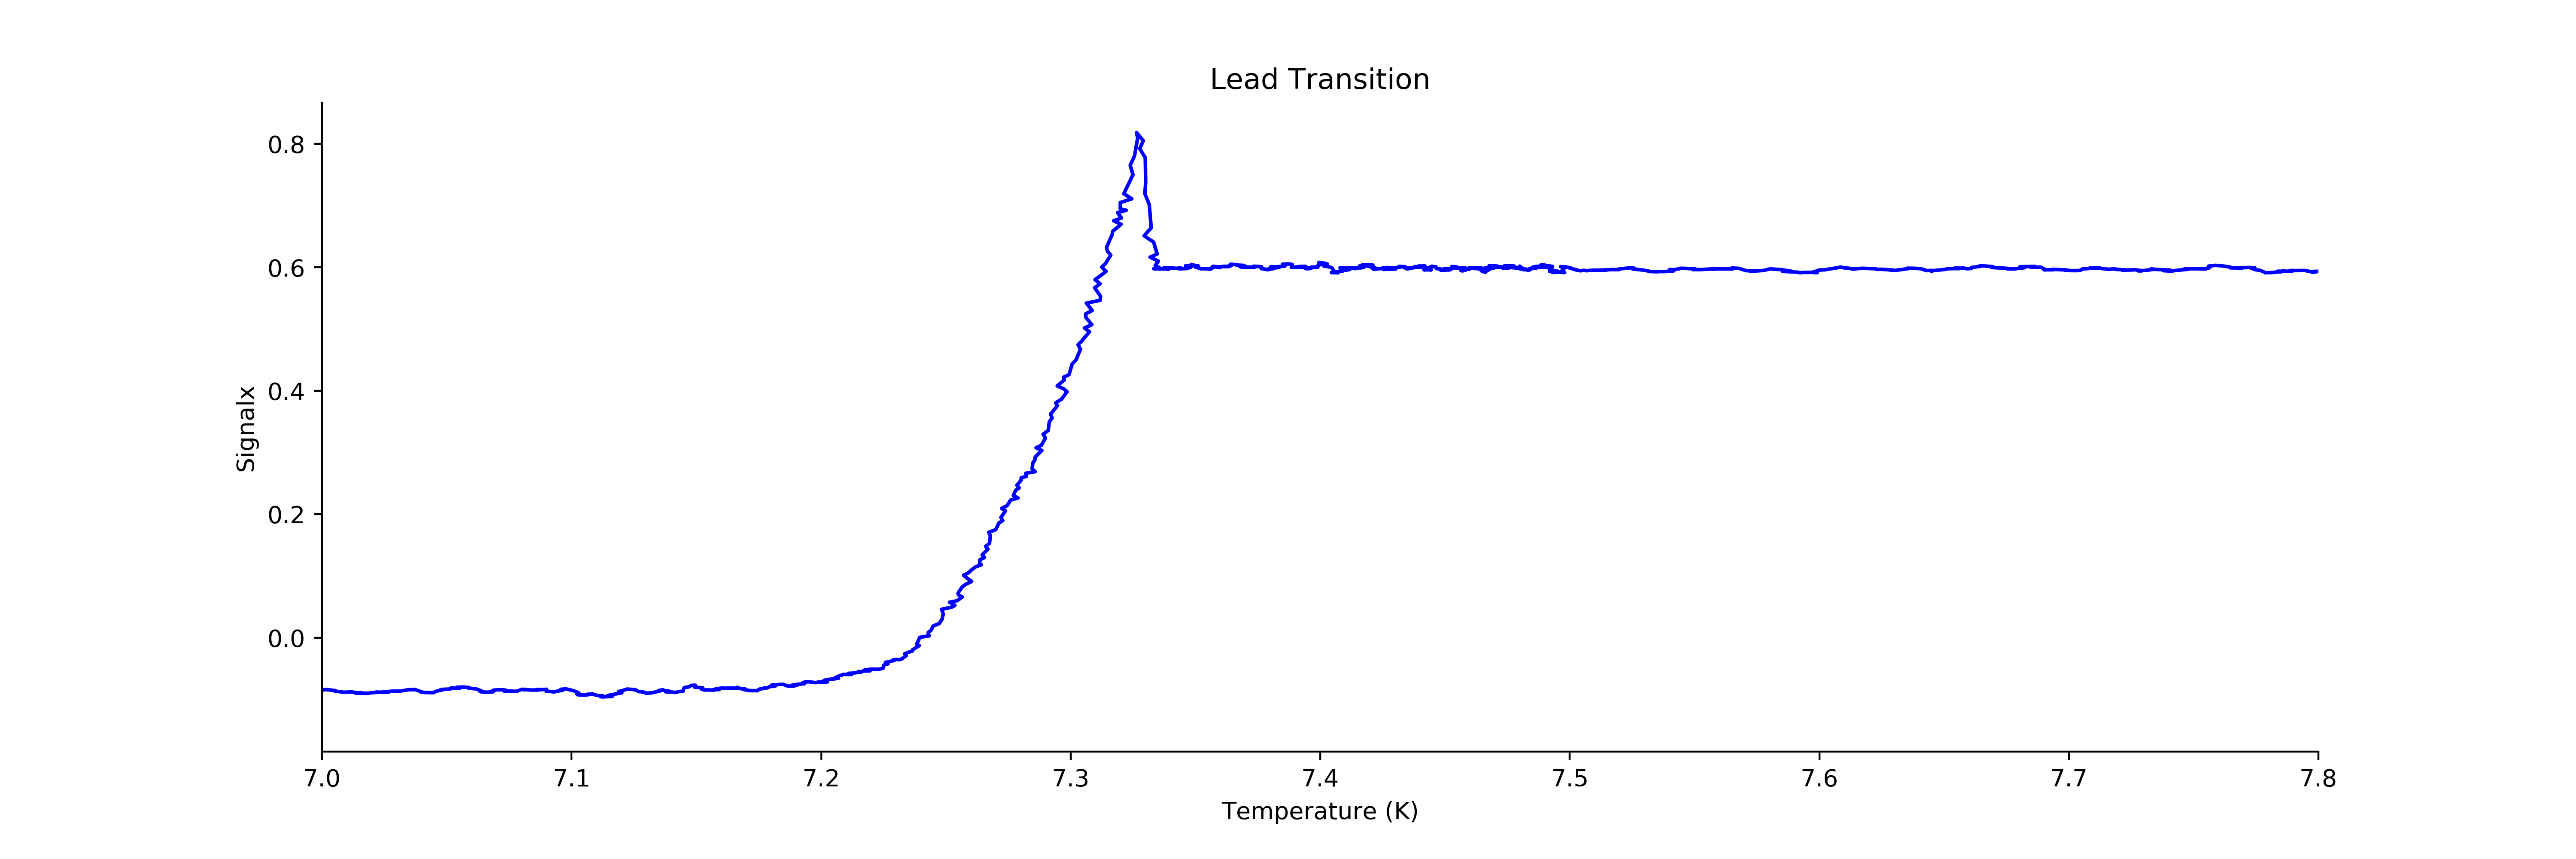
\includegraphics[width=.8\columnwidth]{figures/lead.png}
	\caption{Wiring scheme between coils}
	\label{fig:9}
\end{figure}

The shape is irregular likely due to the setup of the sample coil itself, where the pickup coil wraps around the drive. When the lead goes superconducting, it expels magnetic flux and this causes it to be pushed outward, so more flux will be observed by the pickup coil. As the lead continues to become superconducting, the flux continues to be expelled till it reaches a constant value below the T$_C$. If the drive coil wrapped around the pickup instead, one would not expect a sharp rise before the fall see in Figure \ref{fig:9} and would have a shape as expected from such a transition.

\section{Conclusion and Outlook}

I have developed a modified version of an Indenter cell, which is easier to handle compared to previous versions, while still being able to reach pressures up to 4.5GPa. Up to these pressures, magnetic susceptibility measurements can be made to observe any magnetic transitions that may occur within the sample space. Other types of measurements, such as resistivity are possible as well, but have not been tested in this report.\\

This setup still has the drawback of sensitive wires which need to be protected, often time with stycast from being severed due to the cone seal in Figure \ref{fig:2}. A possible work around for this would be to use thicker wire that can still fit in the sample region, simply with fewer turns. To compensate for the lower magnetic flux that would be produced by the lower number of turns on the drive coil, the current could be increased by an amount that would compensate for the number of turns according to Equation \ref{eq:2}.\\

In the future, other transitions will be measured using this cell, in particular the anti-ferromagnetic transition of FBBO leading to a quantum critical point near 3GPa.\cite{FBBO}

\bibliographystyle{unsrt}
\bibliography{bib}


\end{document}
